\chapter{Strutture della rete}

\section{Obiettivi dell’analisi strutturale}

Dopo aver analizzato la rete dal punto di vista globale e attraverso le misure di centralità, l’attenzione viene ora rivolta alle sue sottostrutture interne. In particolare, questa fase ha lo scopo di individuare gruppi di aeroporti fortemente interconnessi, il nucleo più coeso della rete, le connessioni locali attorno ad alcuni hub rilevanti e la presenza di sottografi completamente connessi.

Per questo motivo l’analisi è stata condotta sulla versione non diretta della rete, costruita a partire dal grafo diretto delle rotte aeree. Tale scelta è coerente con la natura delle tecniche considerate, poiché metodi come community detection, k-core ed ego-network risultano più adatti a una rappresentazione in cui l’interesse principale è la presenza del collegamento, più che il suo orientamento. Prima di procedere, è stato inoltre rimosso il self-loop residuo presente nella rete, così da garantire la compatibilità con gli algoritmi di analisi strutturale.

\section{Community detection}

Per individuare gruppi di aeroporti maggiormente interconnessi tra loro è stato utilizzato l’algoritmo di Louvain, applicato alla largest connected component del grafo non diretto e pesato. Questa procedura consente di partizionare la rete in comunità massimizzando la modularità, ossia favorendo la formazione di gruppi con molte connessioni interne e relativamente poche connessioni verso l’esterno.

L’algoritmo ha individuato un totale di 19 community. Le loro dimensioni risultano molto eterogenee, come mostrato nella Figura~\ref{fig:top_communities}.

\begin{figure}[H]
\centering
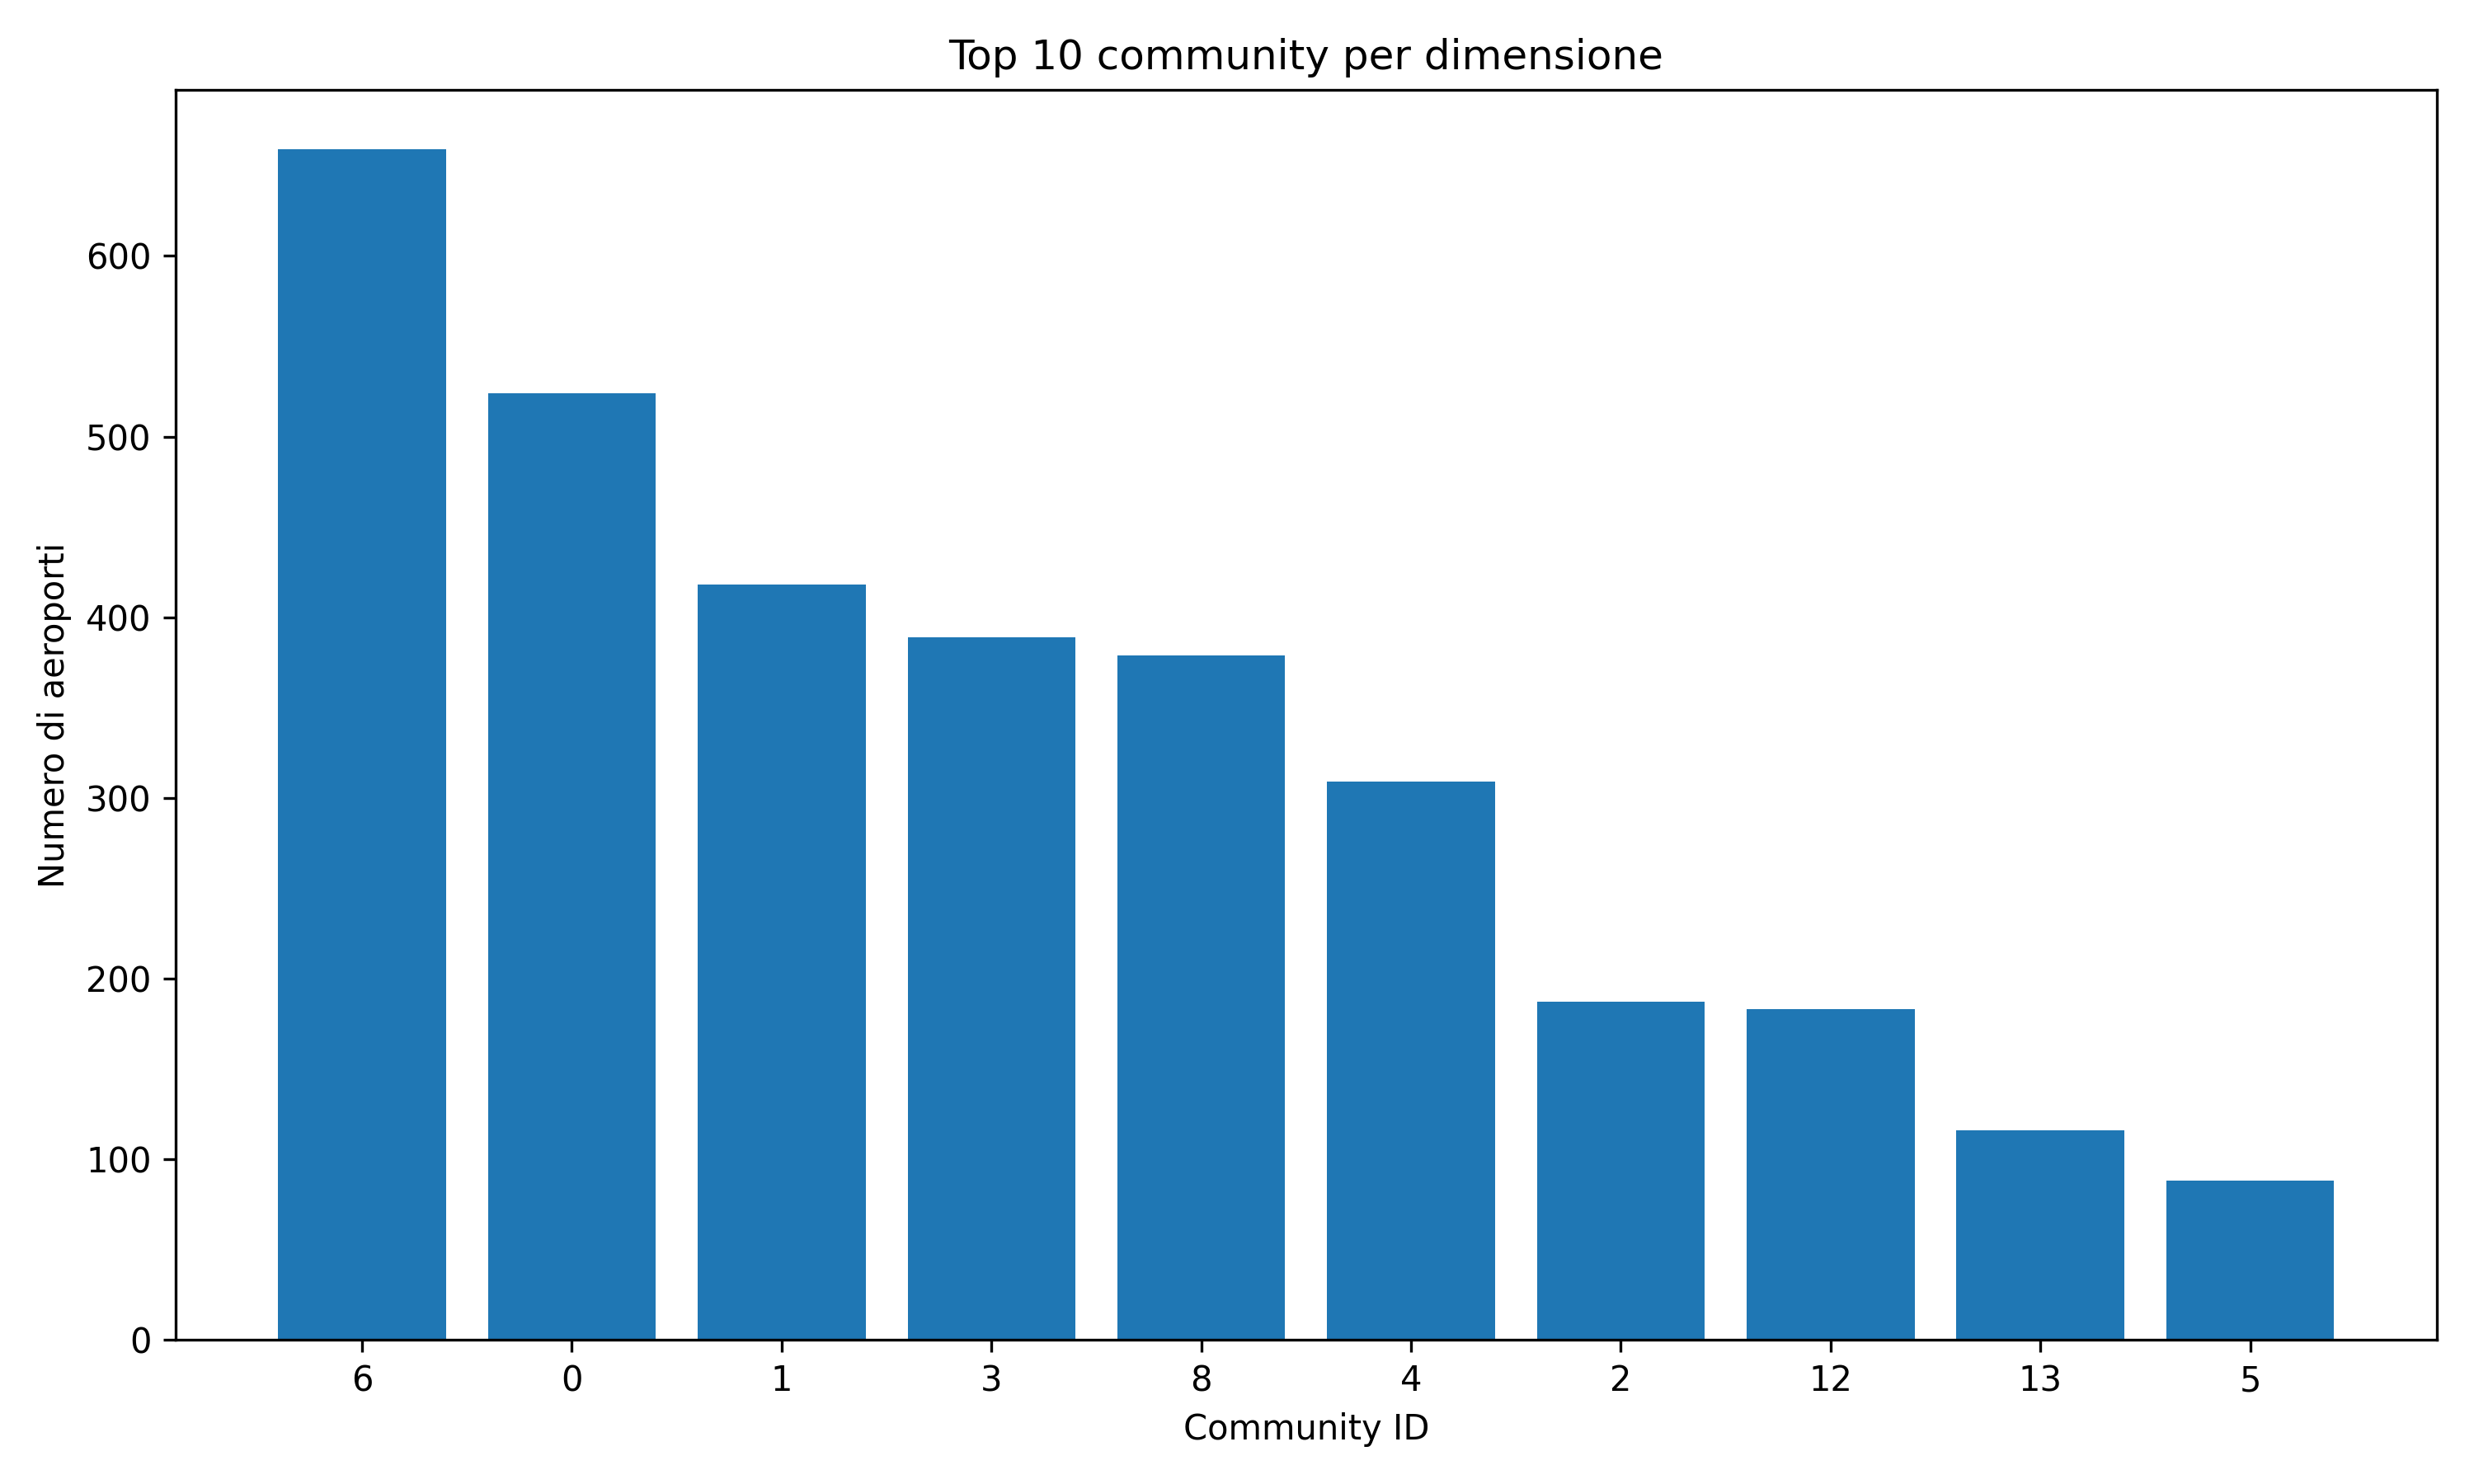
\includegraphics[width=0.9\textwidth]{chapter6/immagini/top10_communities.png}
\caption{Top 10 community per dimensione individuate con l’algoritmo di Louvain.}
\label{fig:top_communities}
\end{figure}

La community più grande è la numero 6 e contiene 659 aeroporti. Tra i primi nodi appartenenti a questa comunità compaiono, ad esempio, ATL, ORD, DFW, DEN, JFK, IAH e PHL, suggerendo una struttura fortemente riconducibile a un sottoinsieme molto integrato del traffico aereo nordamericano.

Le restanti community presentano comunque dimensioni significative: la seconda comunità contiene 524 aeroporti, mentre altre risultano comprese tra circa 300 e 400 nodi. Questo risultato mostra che la rete, pur appartenendo a un sistema globale fortemente interconnesso, presenta una chiara organizzazione interna in blocchi di aeroporti con elevata coesione.

Per affiancare al dato quantitativo una rappresentazione visiva dell’organizzazione interna della rete, è stata generata anche una visualizzazione globale della largest connected component, colorata in base alla community di appartenenza.

\begin{figure}[H]
\centering
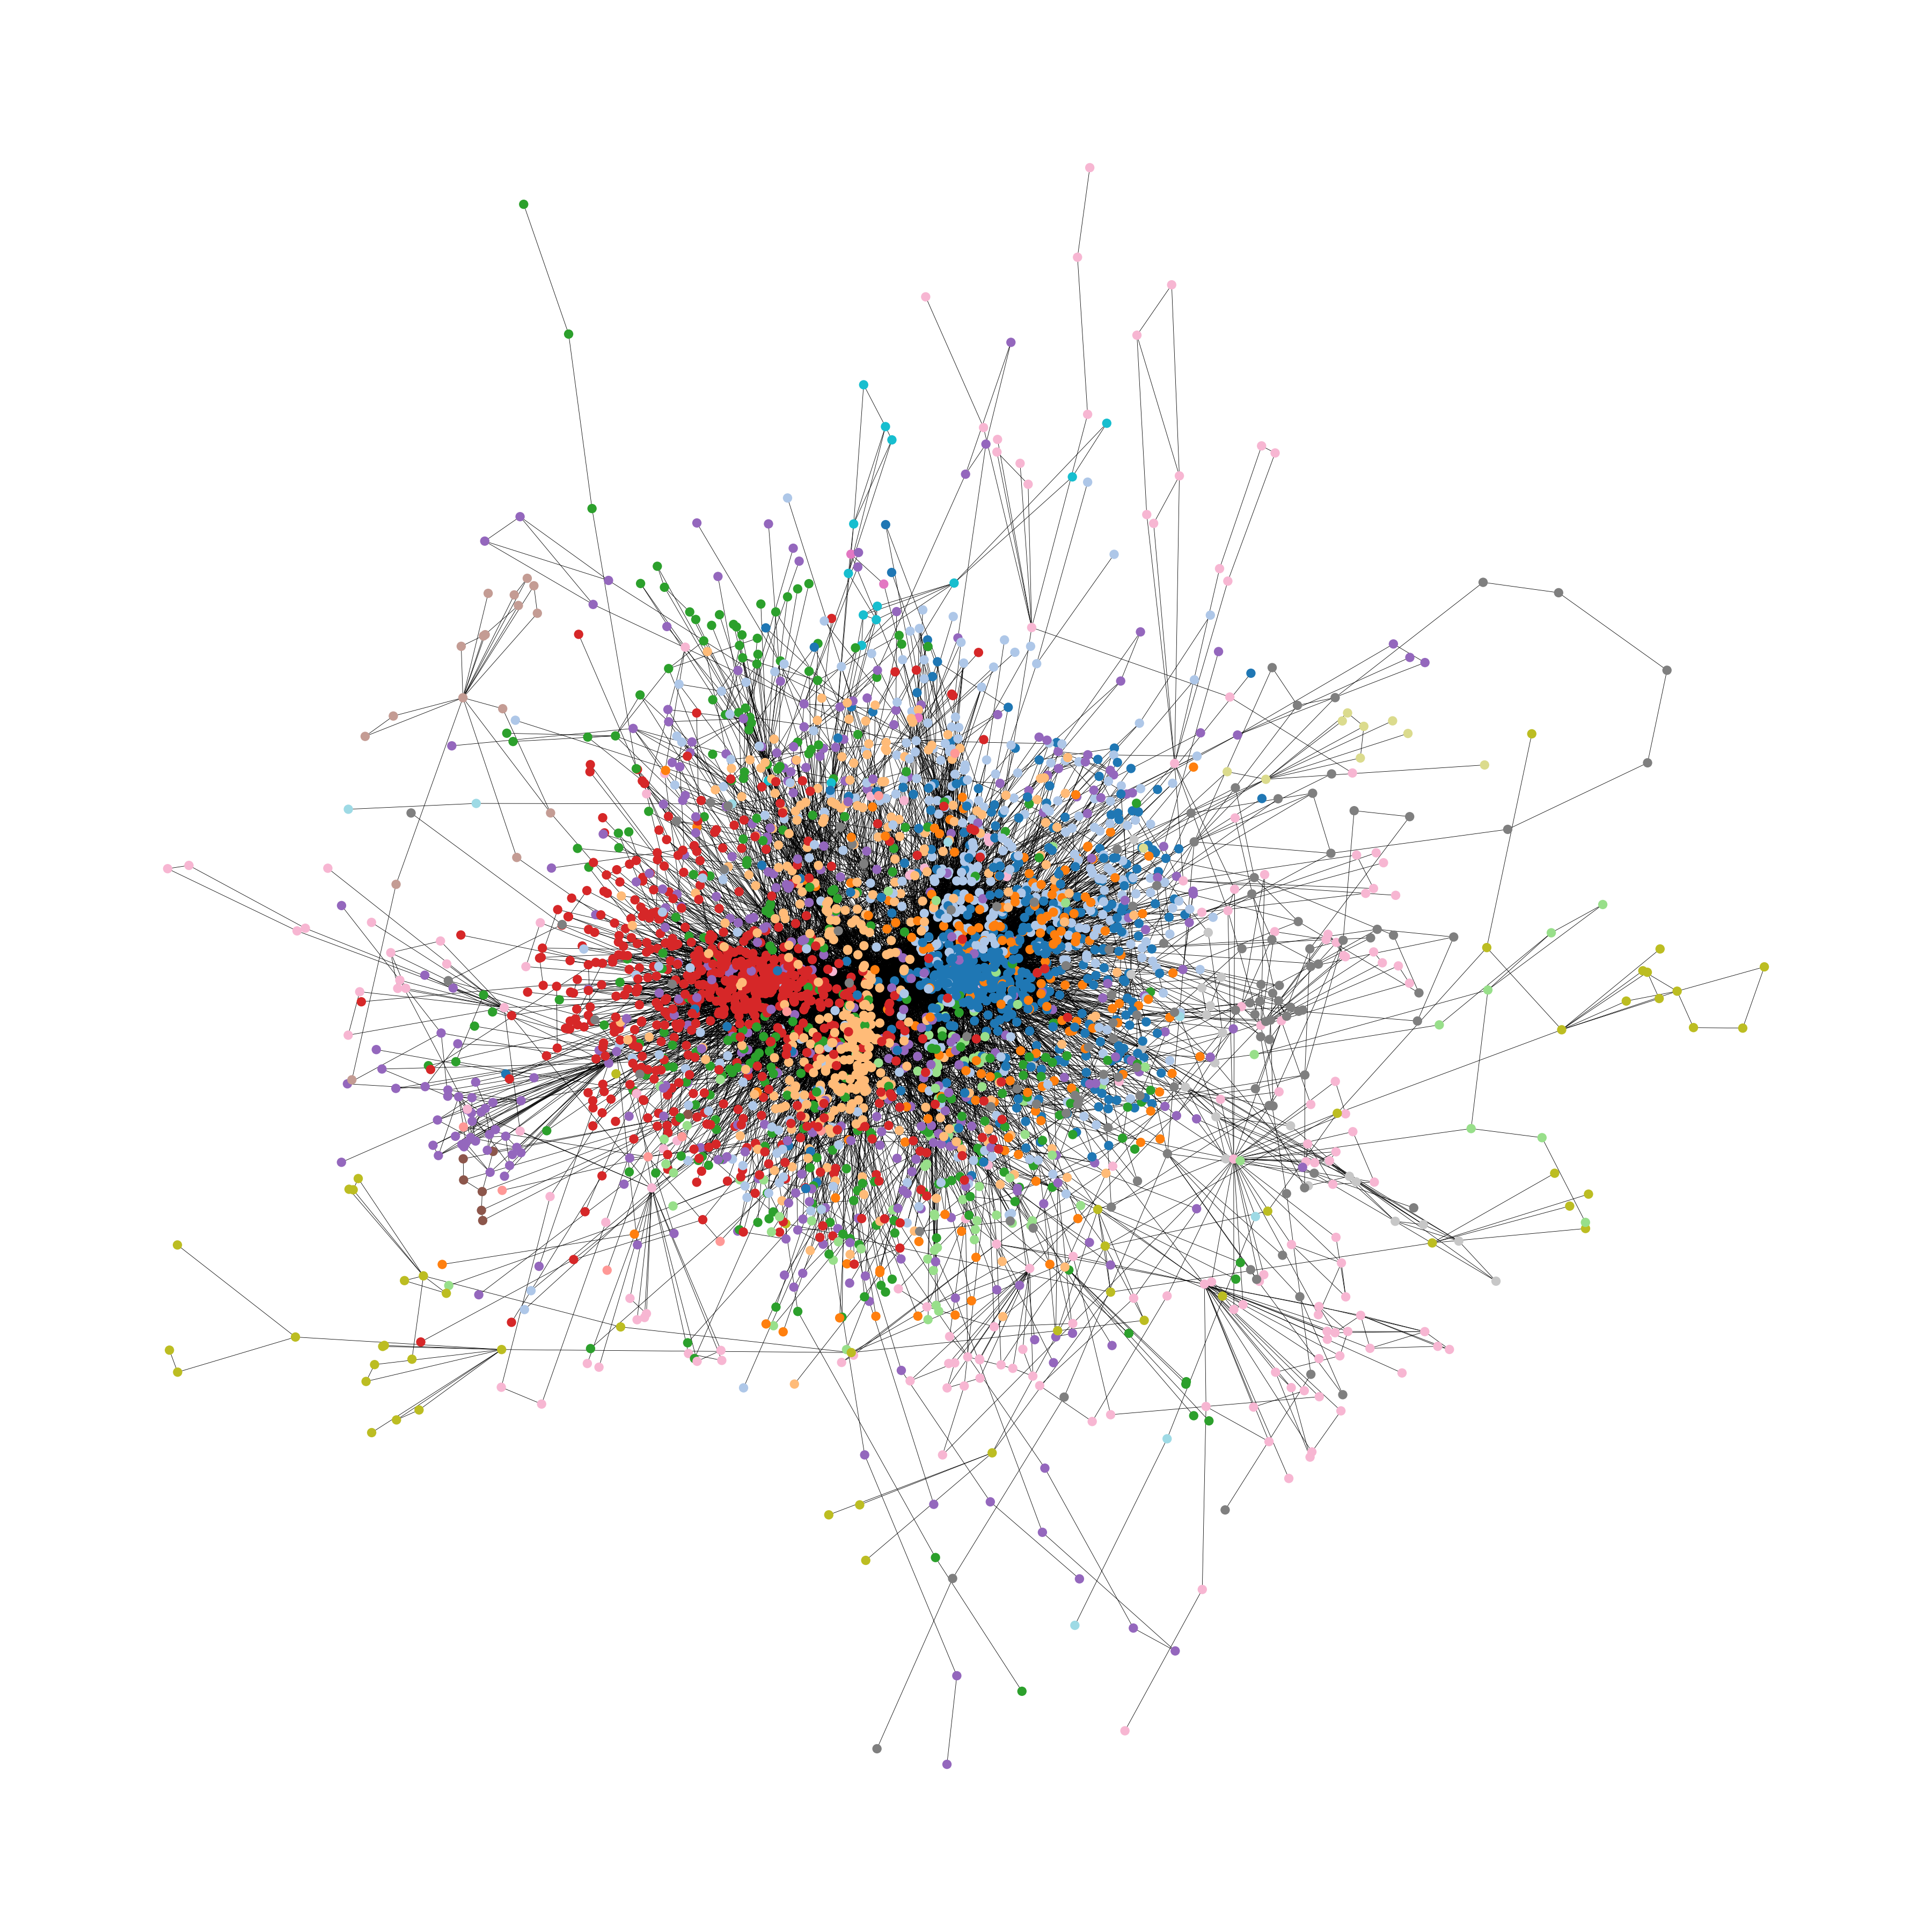
\includegraphics[width=0.9\textwidth]{chapter6/immagini/community_colored_graph.png}
\caption{Visualizzazione della rete colorata in base alla partizione in community.}
\label{fig:community_colored_graph}
\end{figure}

La Figura~\ref{fig:community_colored_graph} permette di osservare come le comunità non siano distribuite in modo casuale, ma tendano a occupare porzioni riconoscibili della rete. Pur restando una struttura fortemente interconnessa, emergono infatti aree con maggiore densità interna e con una certa separazione rispetto alle altre, coerenti con la logica della community detection.

Per approfondire ulteriormente questo aspetto, sono stati rappresentati anche i sottografi relativi alle prime tre community per dimensione.

\begin{figure}[H]
\centering
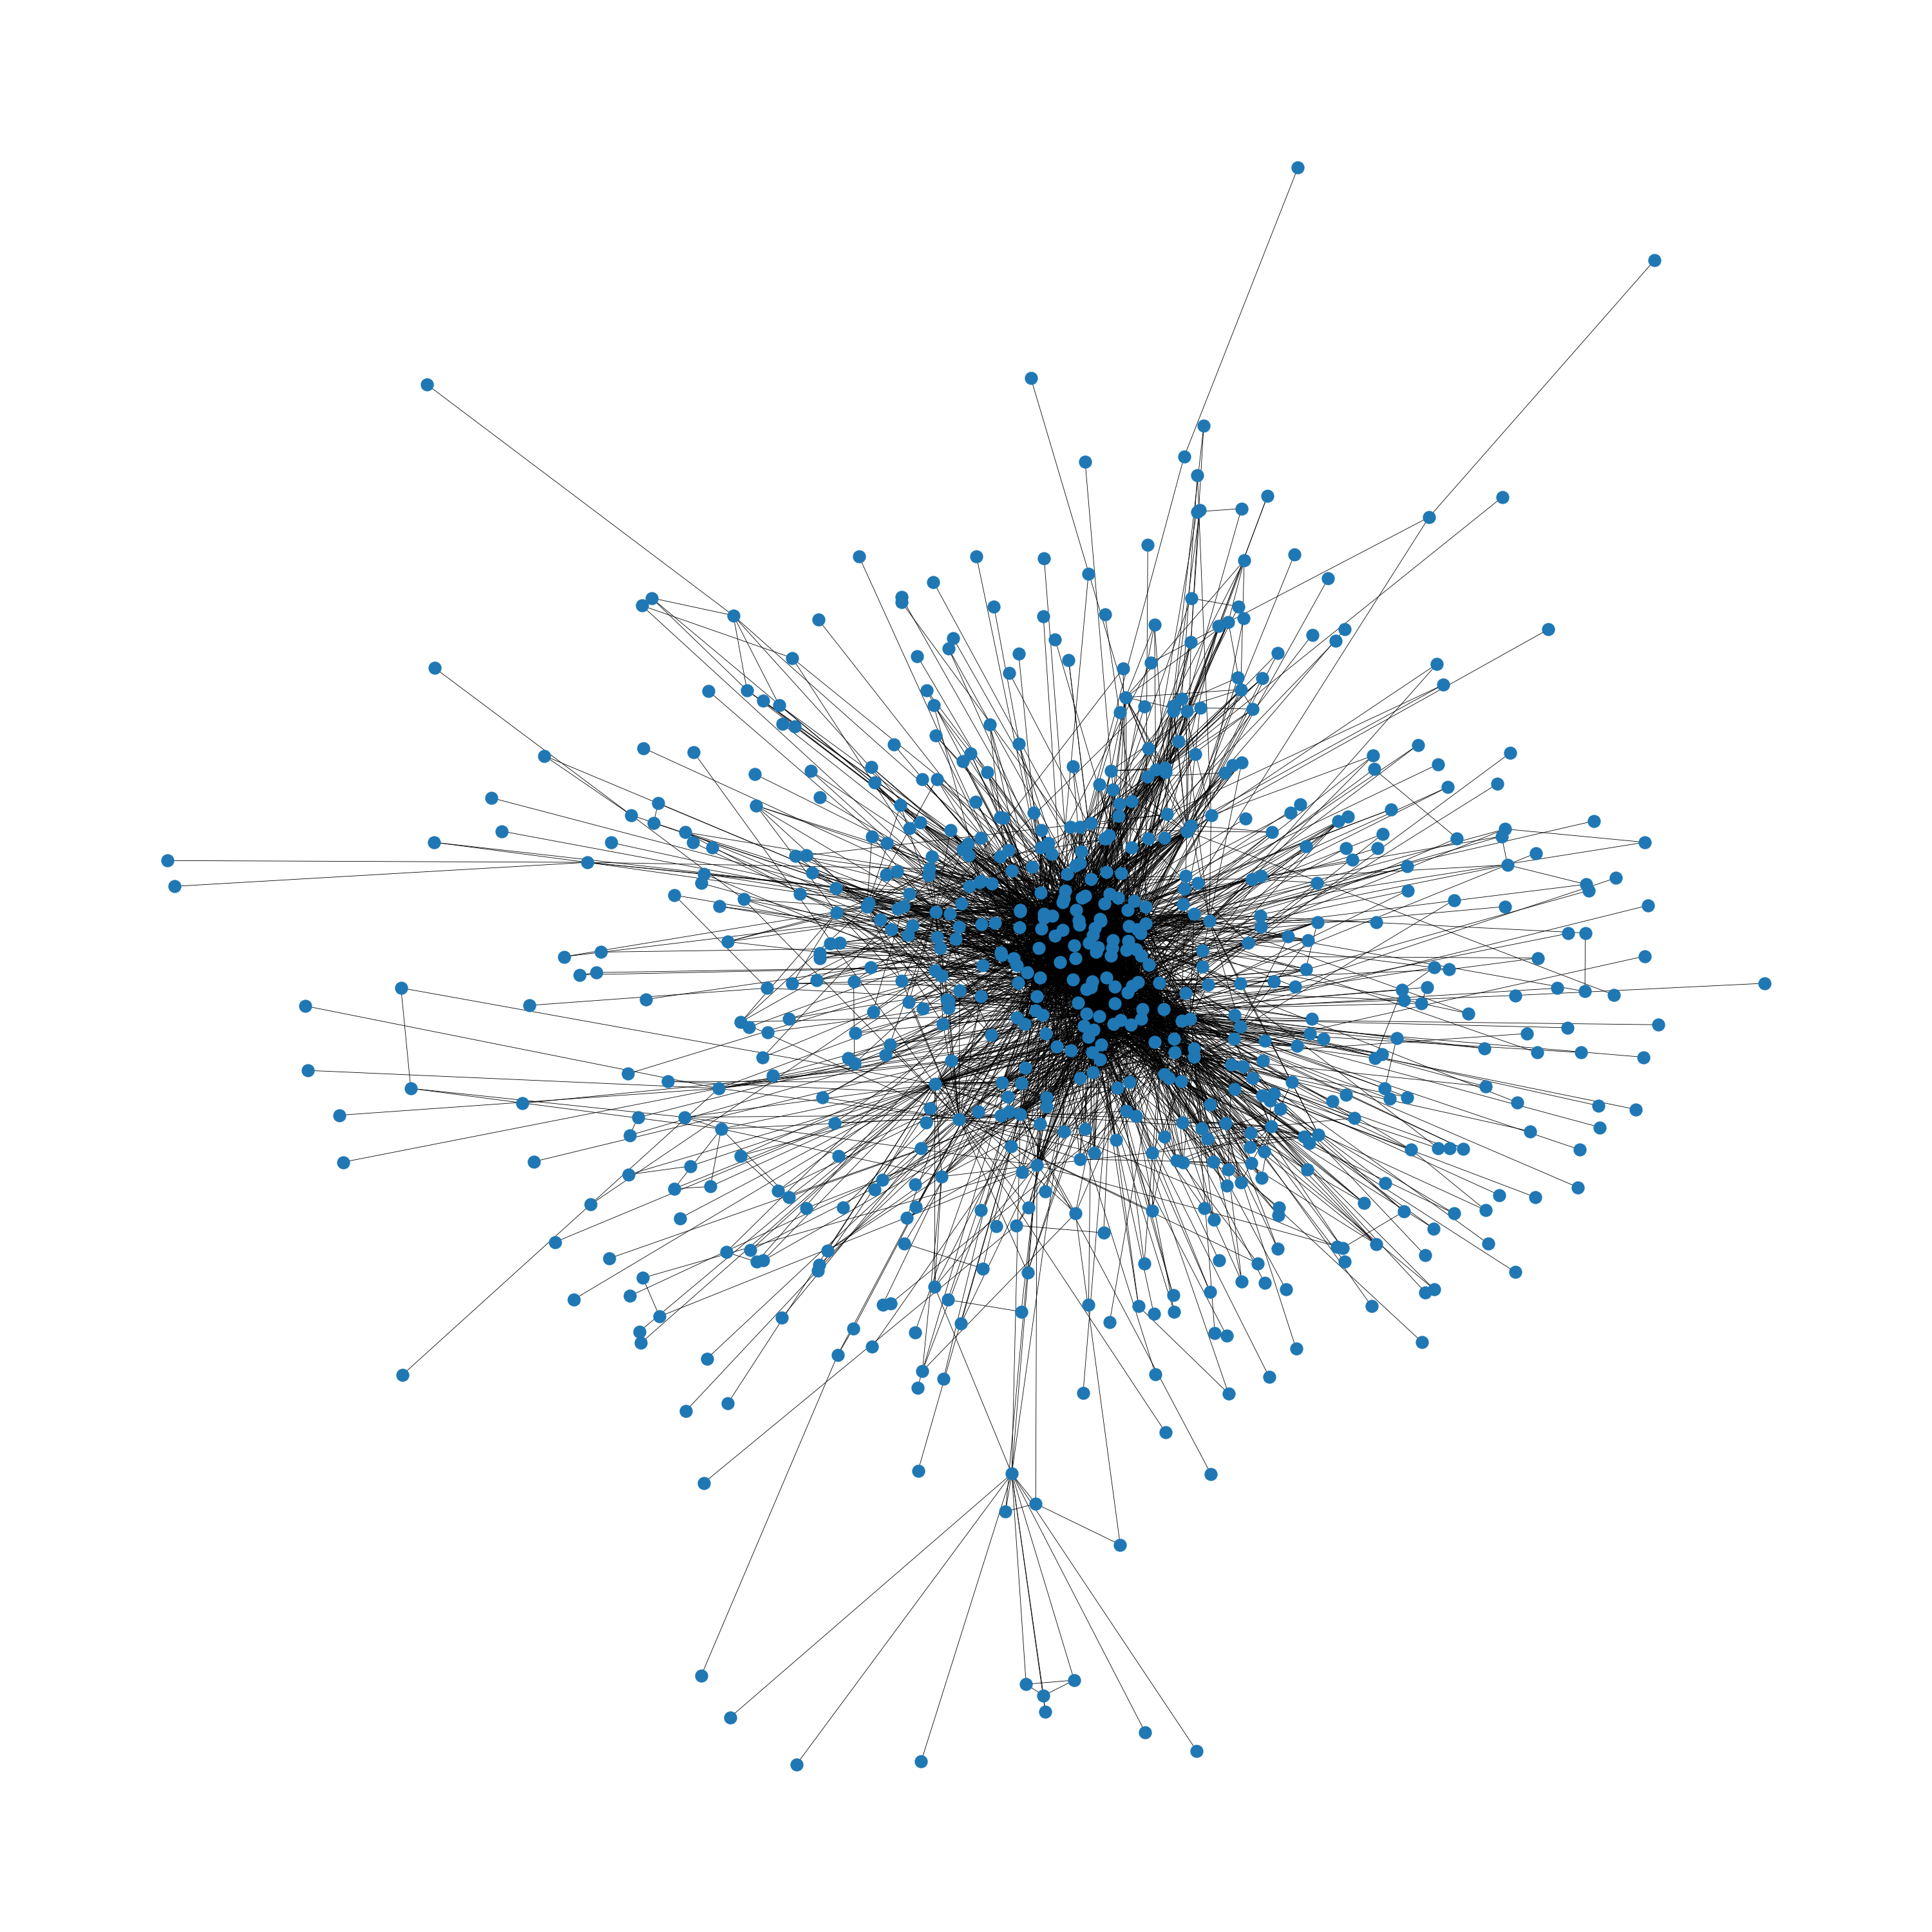
\includegraphics[width=0.9\textwidth]{chapter6/immagini/community_1_subgraph.png}
\caption{Sottografo della prima community per dimensione.}
\label{fig:community_1_subgraph}
\end{figure}

\begin{figure}[H]
\centering
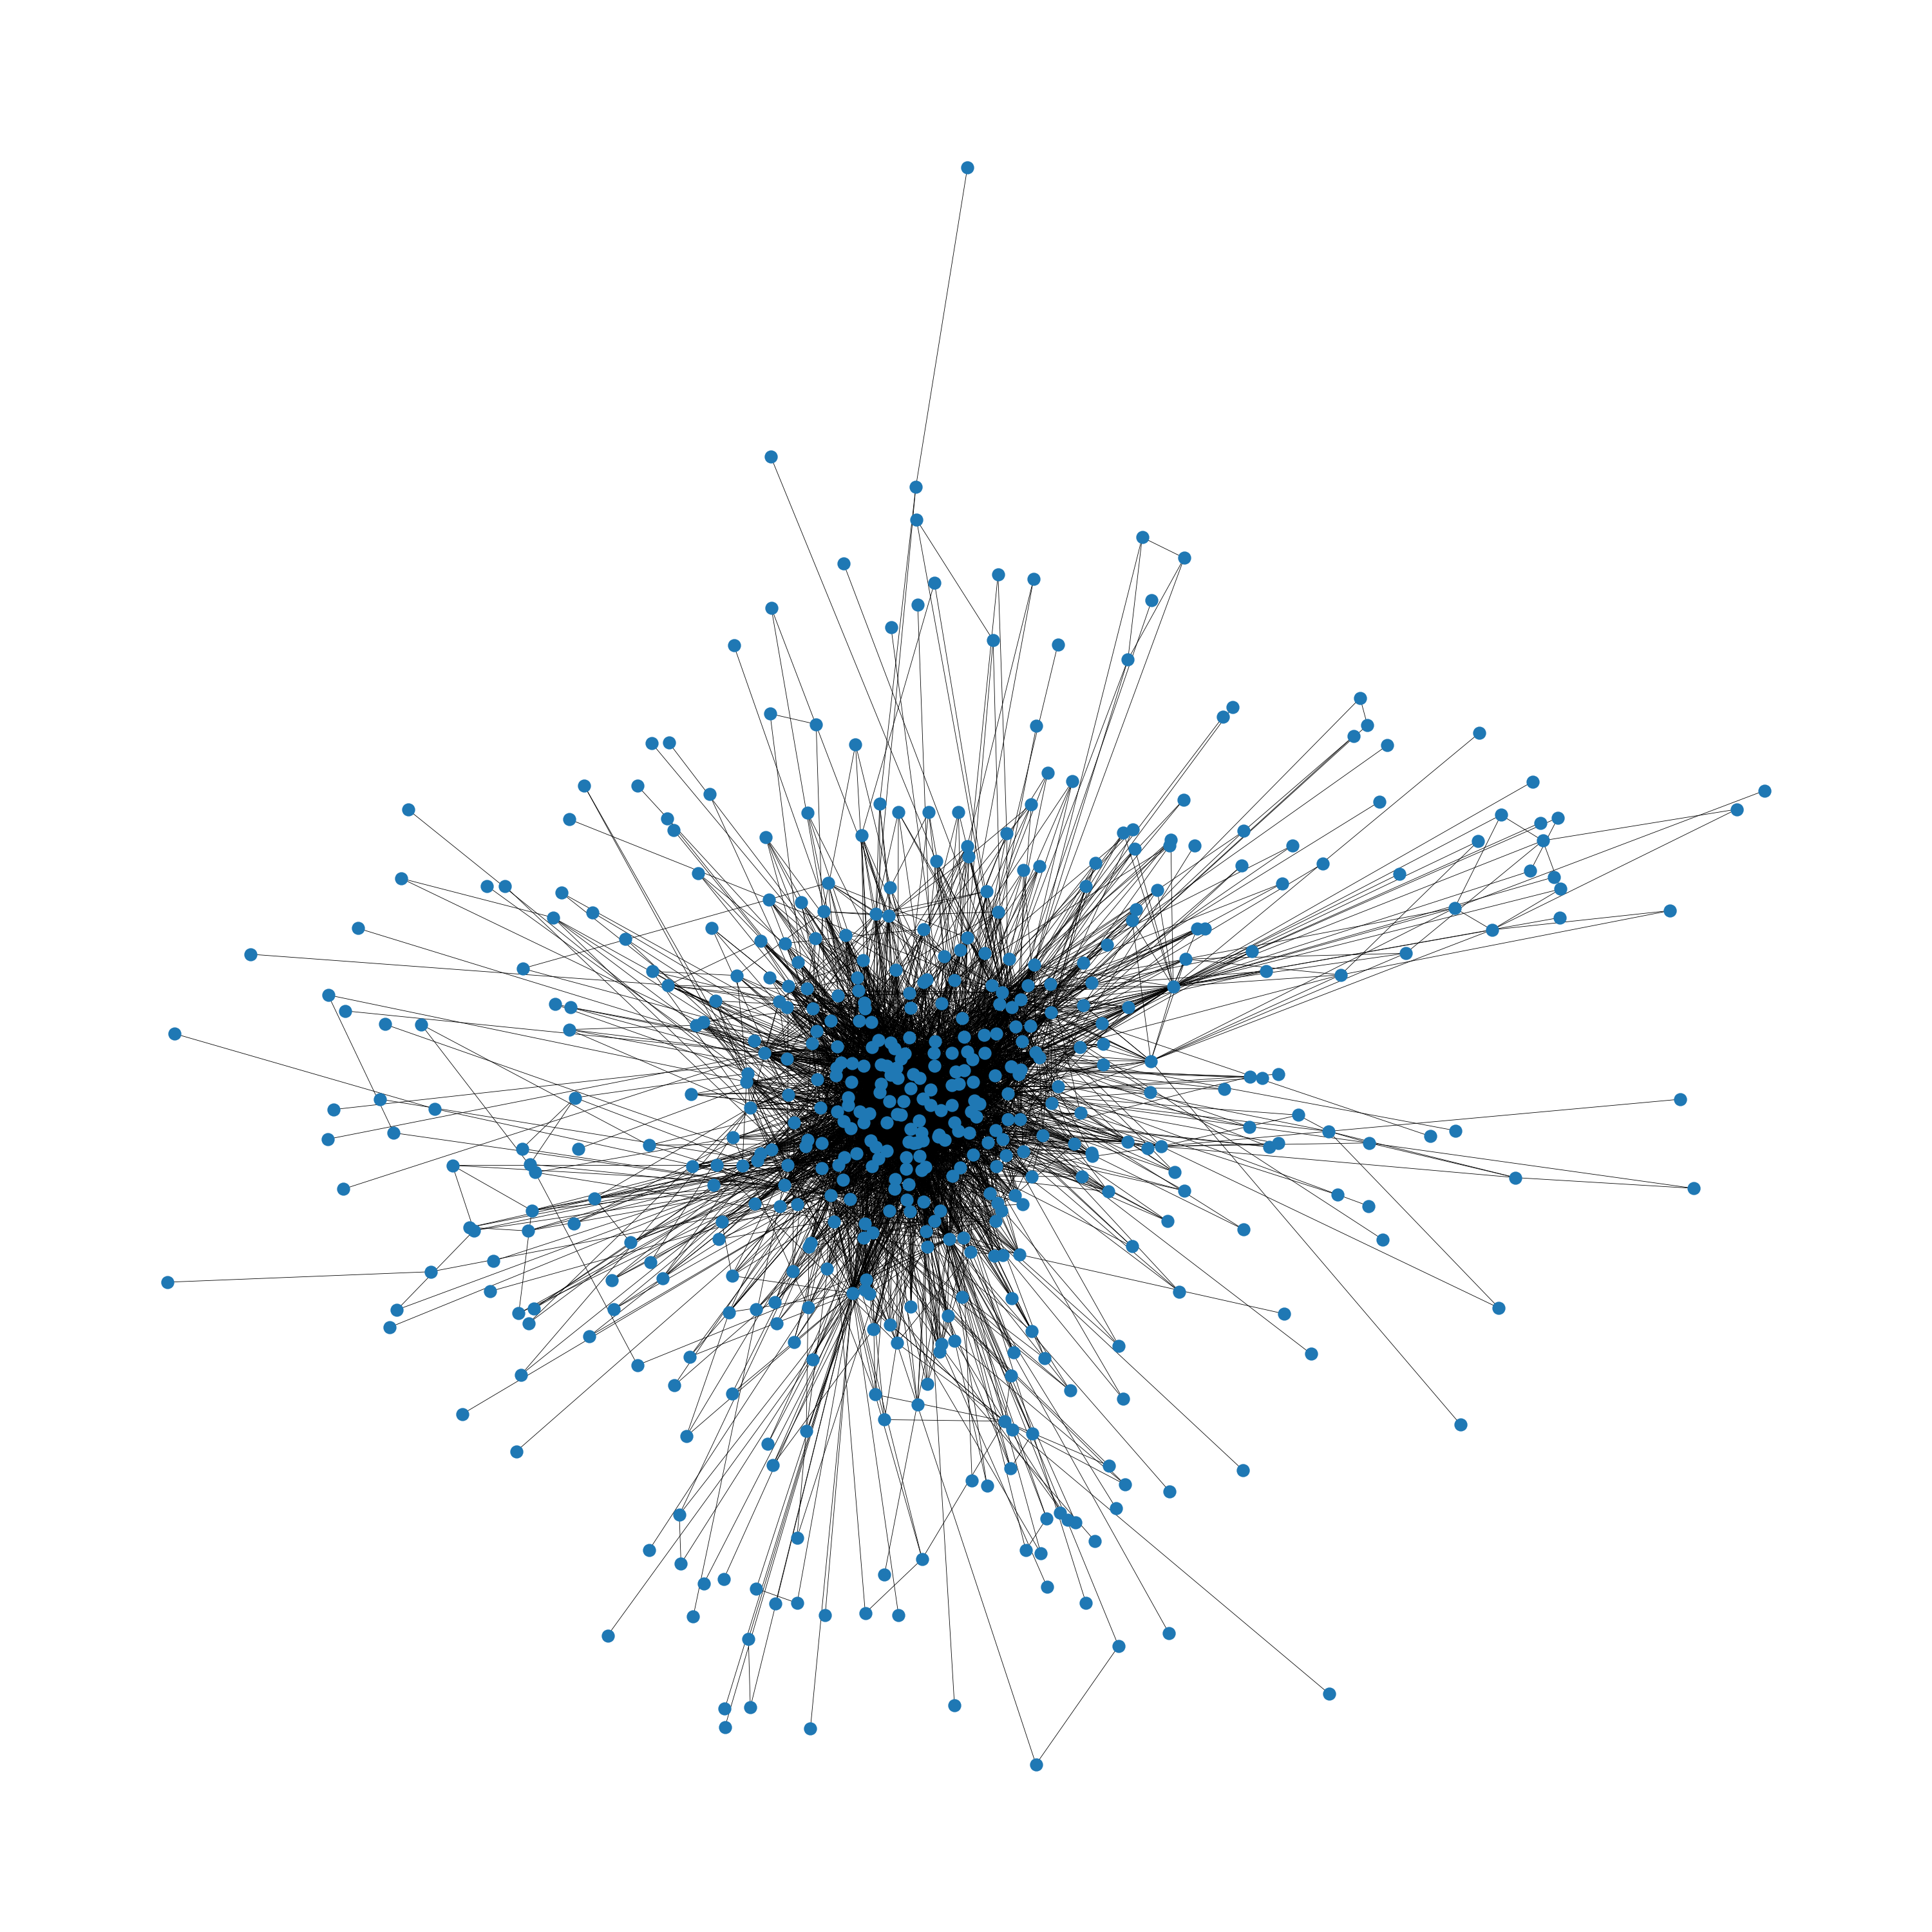
\includegraphics[width=0.9\textwidth]{chapter6/immagini/community_2_subgraph.png}
\caption{Sottografo della seconda community per dimensione.}
\label{fig:community_2_subgraph}
\end{figure}

\begin{figure}[H]
\centering
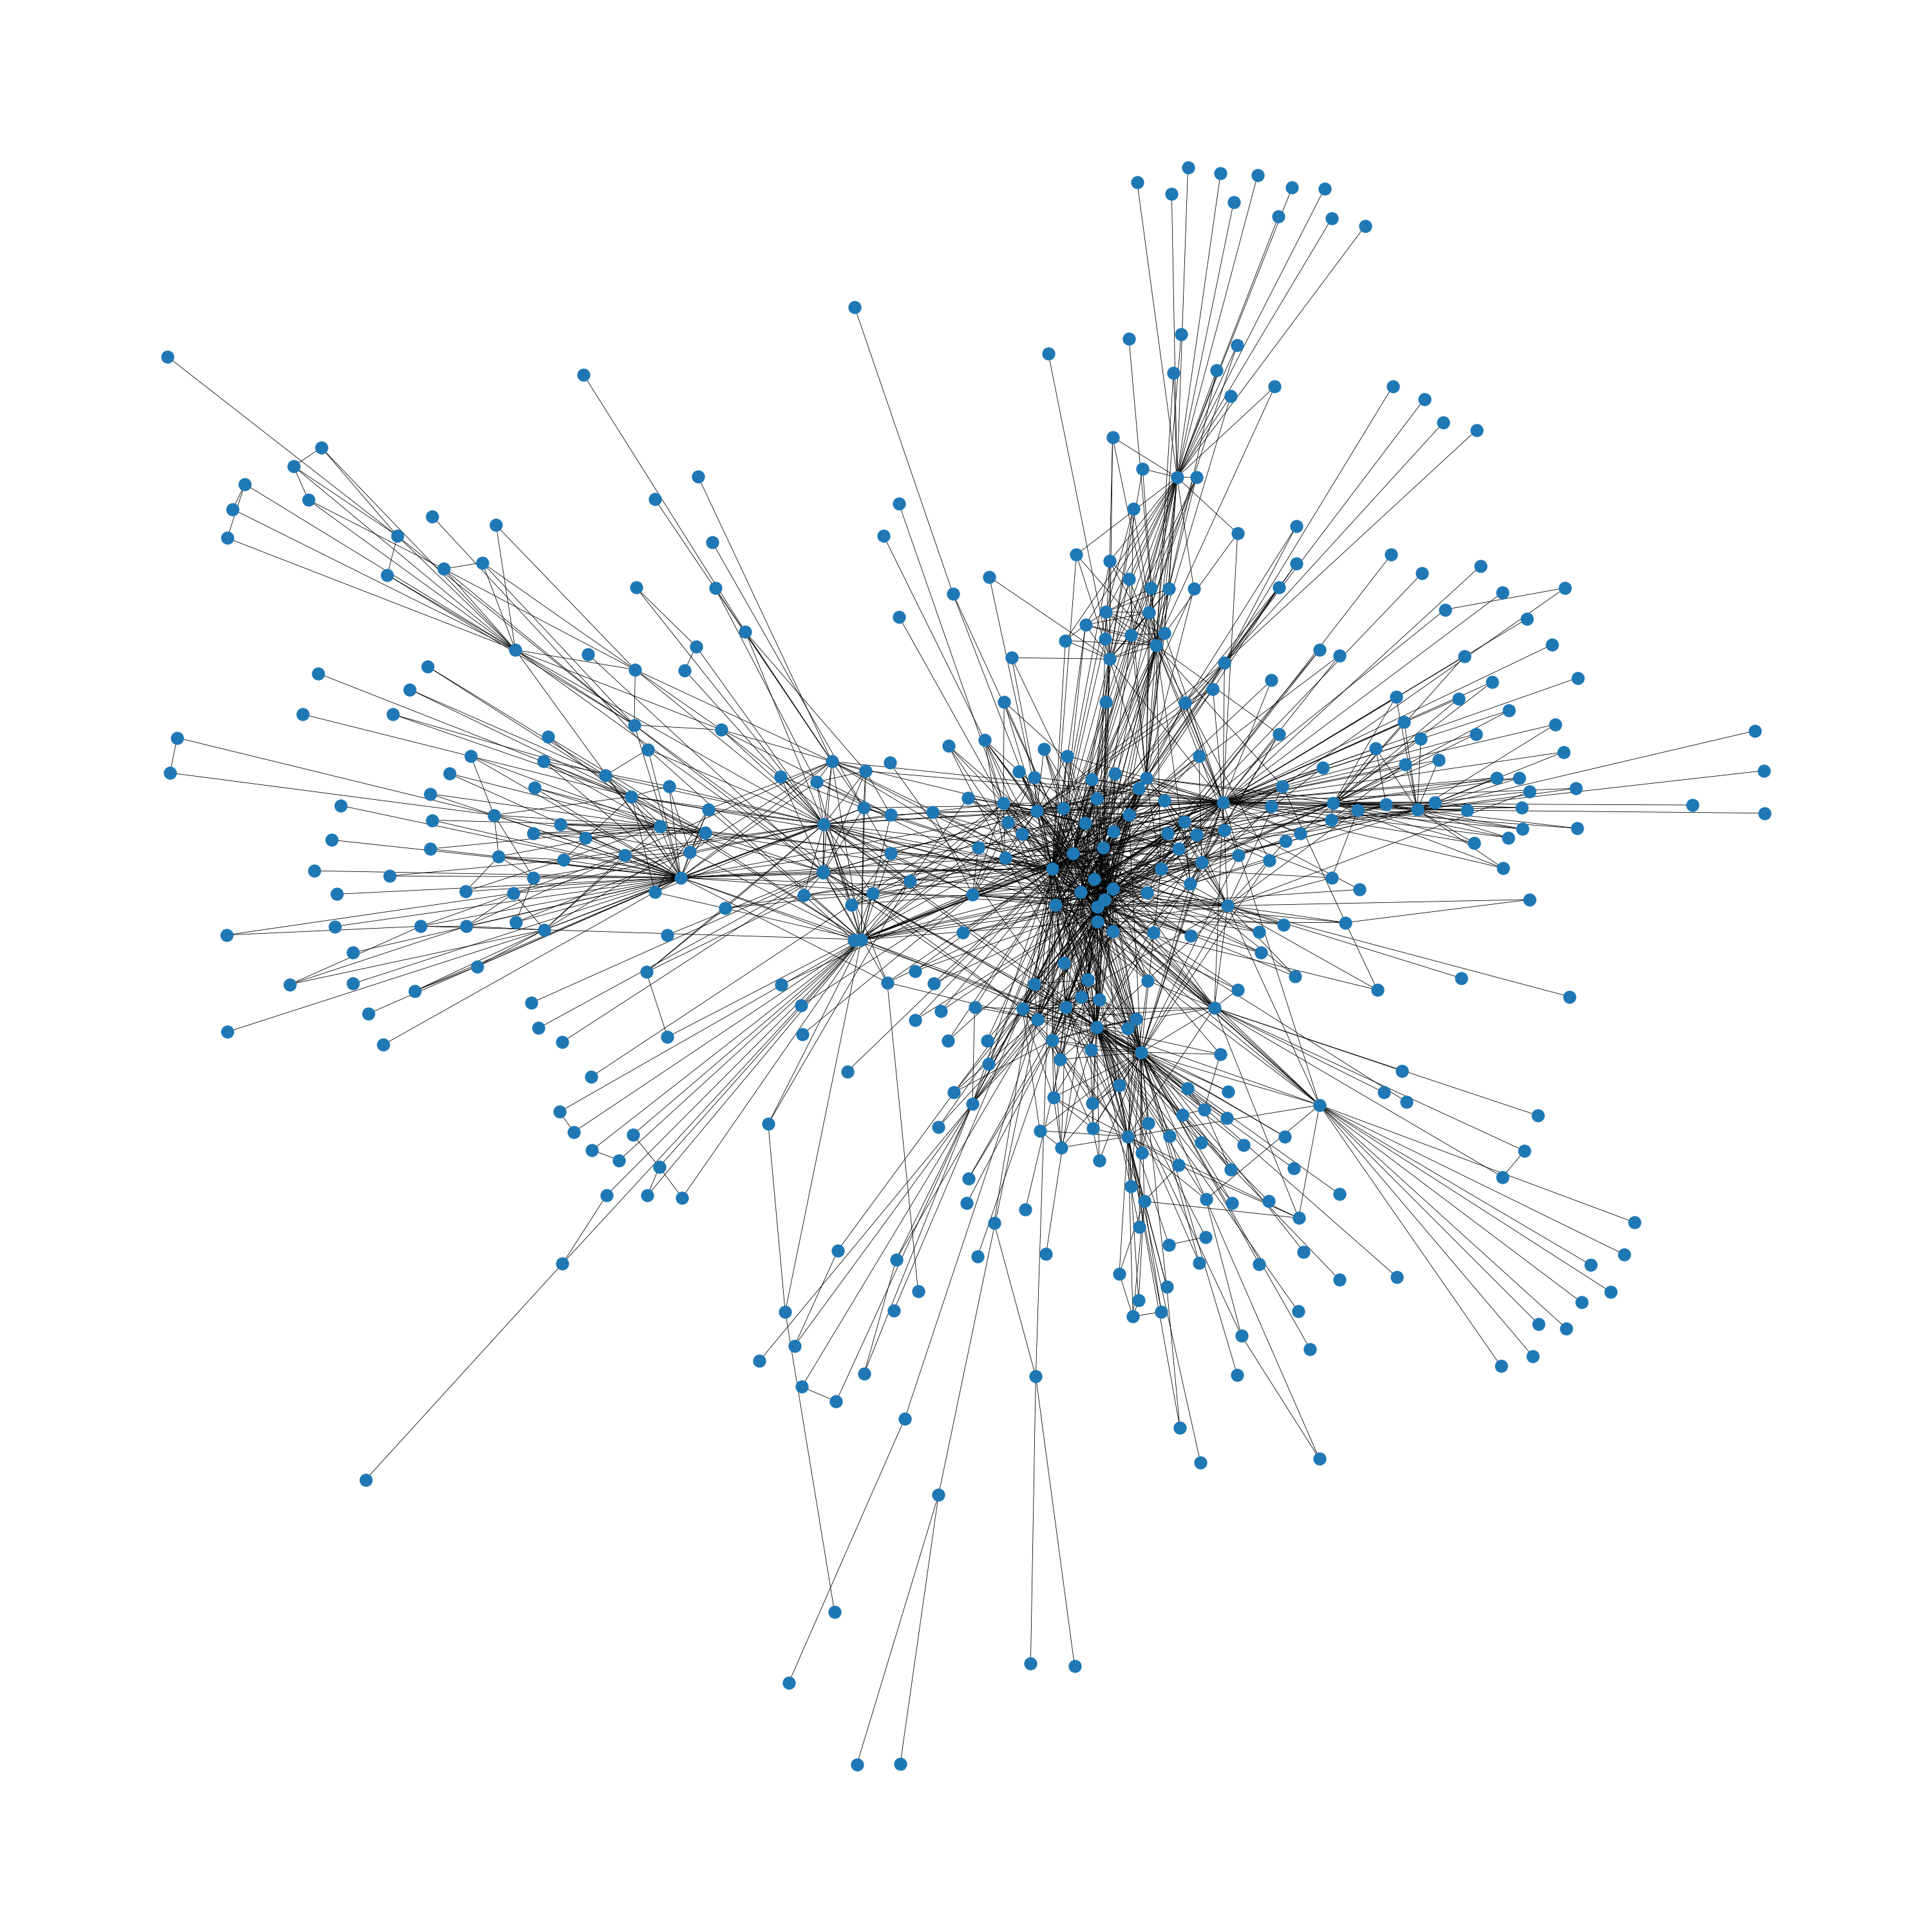
\includegraphics[width=0.9\textwidth]{chapter6/immagini/community_3_subgraph.png}
\caption{Sottografo della terza community per dimensione.}
\label{fig:community_3_subgraph}
\end{figure}

Le Figure~\ref{fig:community_1_subgraph}, \ref{fig:community_2_subgraph} e \ref{fig:community_3_subgraph} mostrano che le comunità principali possiedono strutture interne differenti. Alcune appaiono più raccolte e dense, altre più distribuite e articolate. Questa osservazione rafforza l’idea che la rete aeroportuale non sia composta da gruppi uniformi, ma da sottosistemi con configurazioni interne anche molto diverse.

\section{Analisi del k-core}

Per approfondire il livello di coesione interna della rete è stata effettuata l’analisi del \textit{k-core}. Questa tecnica consente di individuare sottografi in cui ogni nodo è connesso ad almeno \(k\) altri nodi appartenenti allo stesso sottografo. Maggiore è il valore di \(k\), più il nucleo individuato risulta denso e strutturalmente coeso.

Nel caso in esame, il massimo valore di core number risulta pari a 31. Il massimo k-core contiene 93 aeroporti e 2257 archi, rappresentando quindi il cuore più denso e interconnesso dell’intera rete.

\begin{figure}[H]
\centering
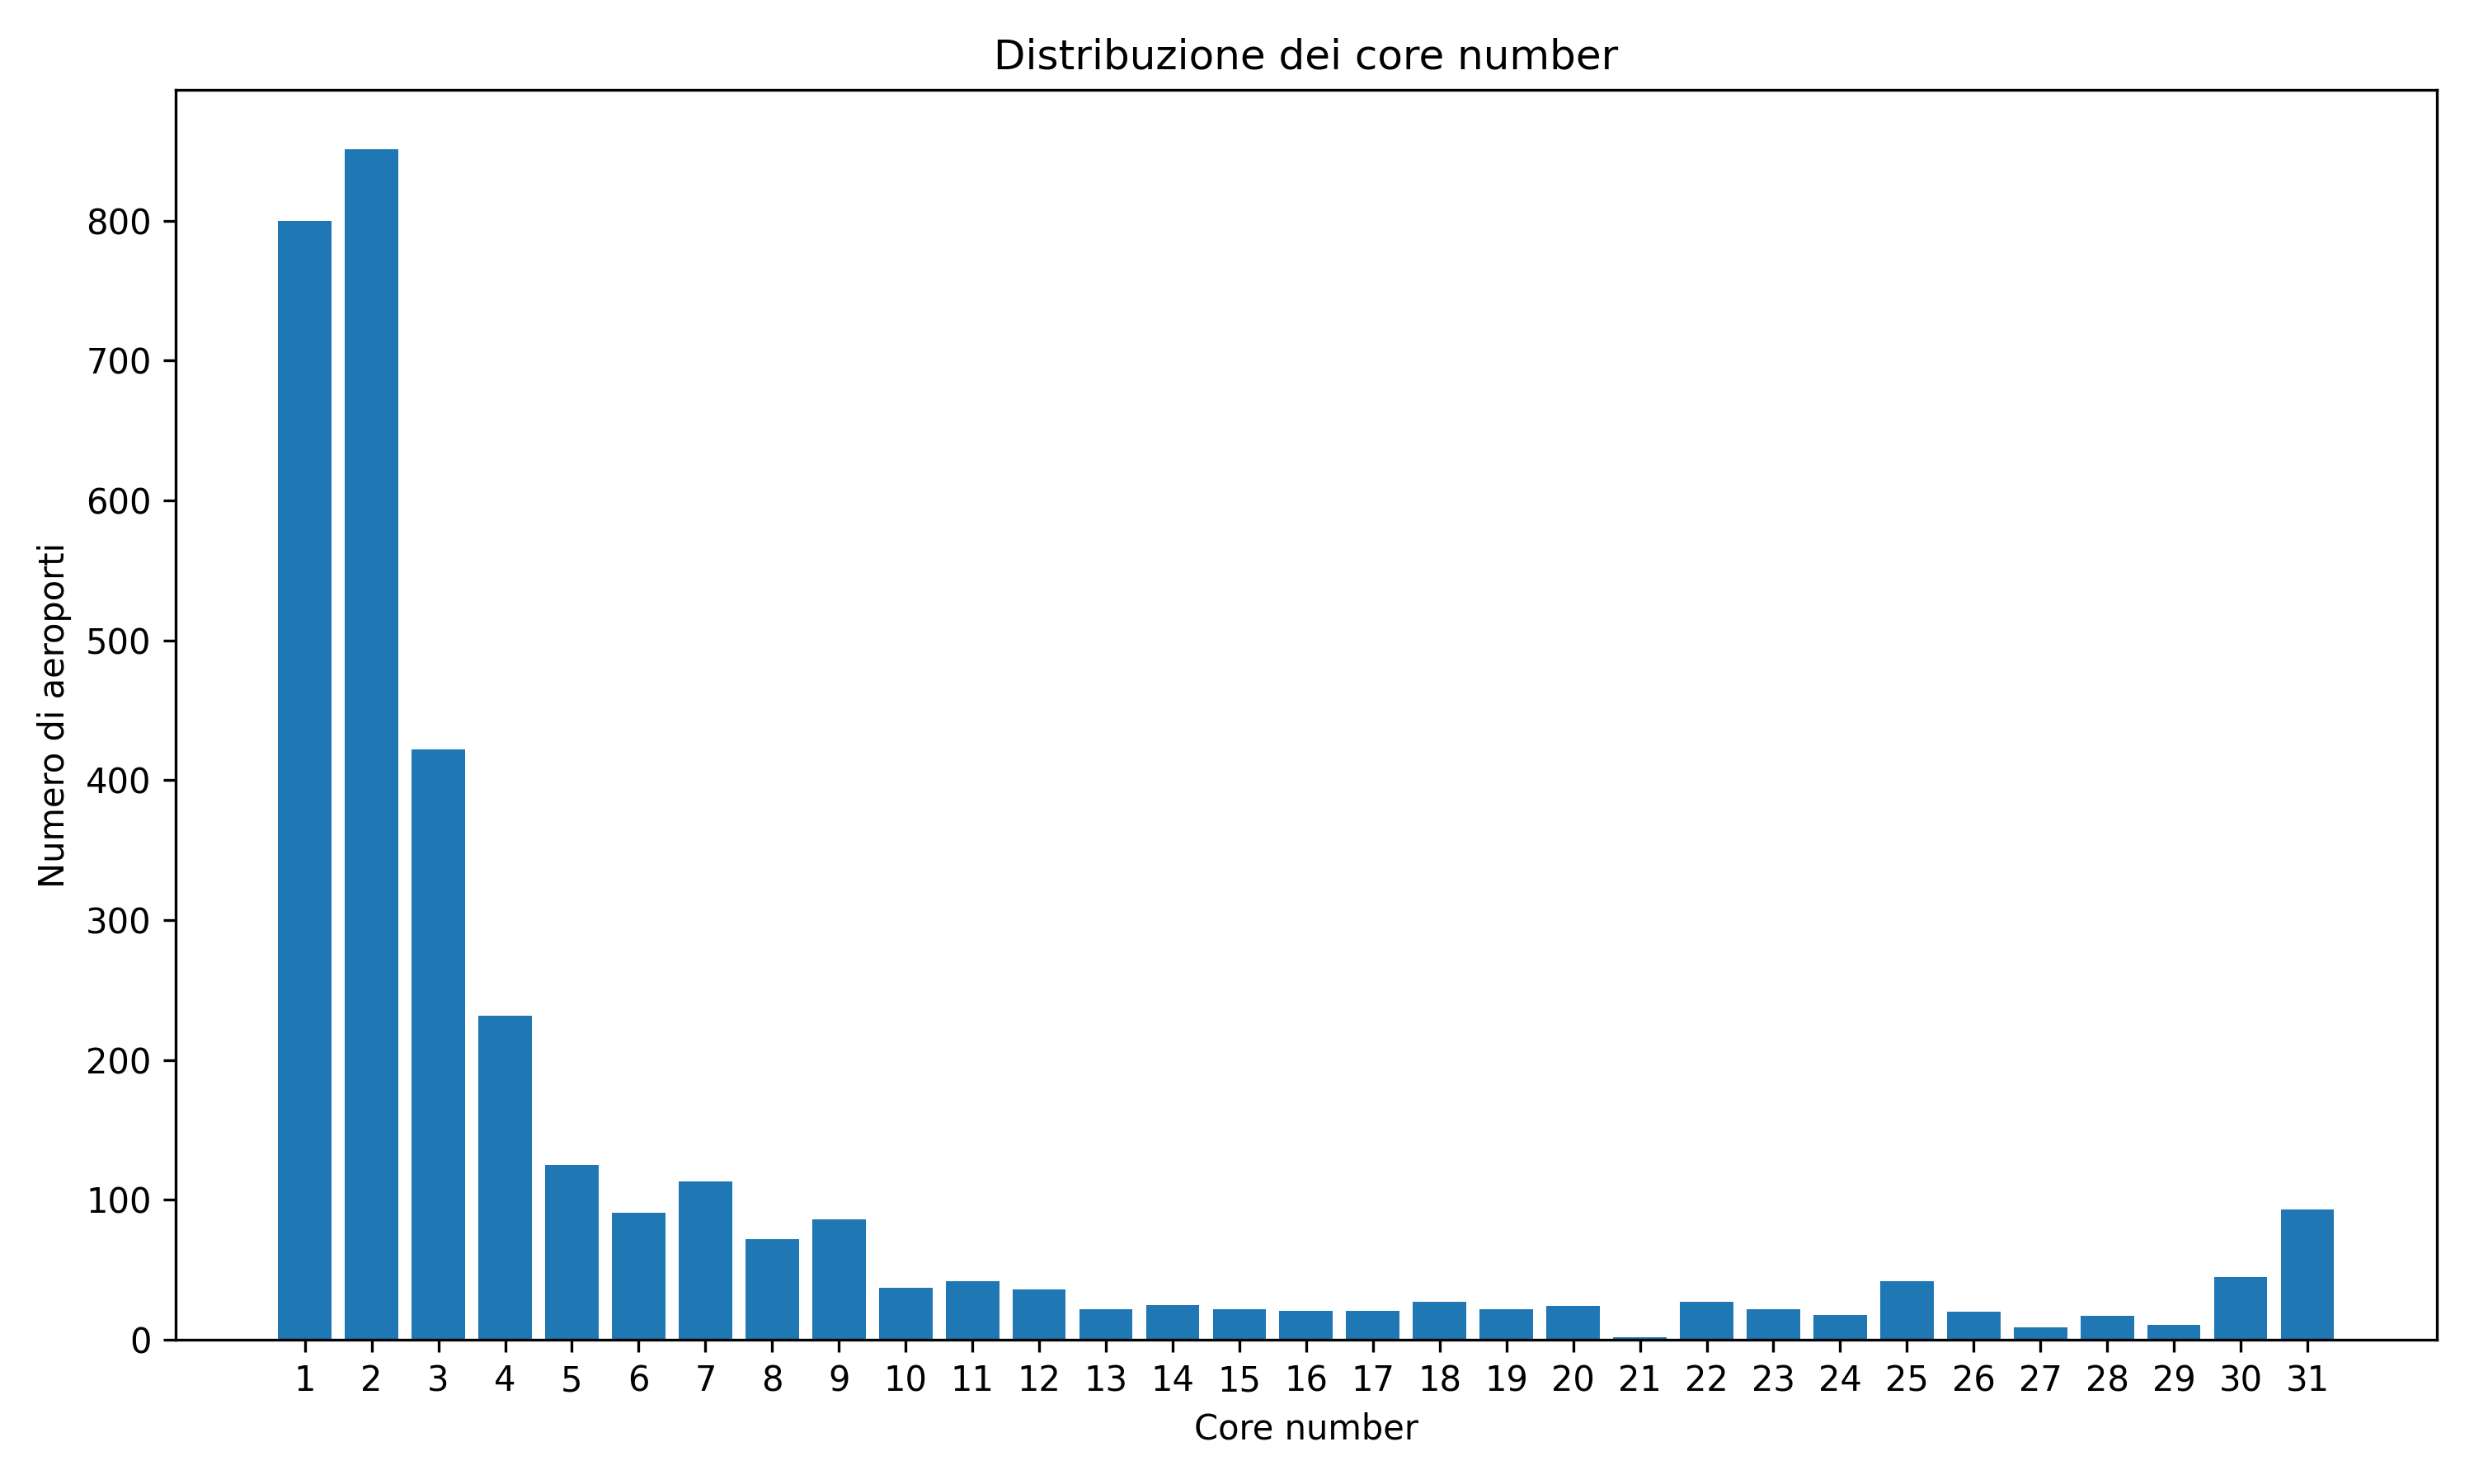
\includegraphics[width=0.9\textwidth]{chapter6/immagini/core_distribution.png}
\caption{Distribuzione dei core number nel grafo non diretto principale.}
\label{fig:core_distribution}
\end{figure}

La Figura~\ref{fig:core_distribution} mostra la distribuzione dei core number tra i nodi della rete. La maggior parte degli aeroporti si concentra sui valori più bassi, mentre un numero progressivamente minore di nodi raggiunge valori elevati, fino al massimo pari a 31. Questo andamento è coerente con quanto osservato nei capitoli precedenti: pochi aeroporti appartengono al nucleo più fortemente coeso, mentre molti altri occupano posizioni più periferiche.

Tra i nodi appartenenti al massimo k-core compaiono aeroporti come LUX, MAD, DBV, ACE, BGY, CTA, TLS, CGN, WAW, DUS, BRU ed EDI. Si tratta di un insieme di nodi fortemente integrati, che può essere interpretato come il nucleo strutturale più stabile della rete.

Per visualizzare in modo diretto questo sottografo altamente coeso, è stata prodotta anche la rappresentazione del massimo k-core.

\begin{figure}[H]
\centering
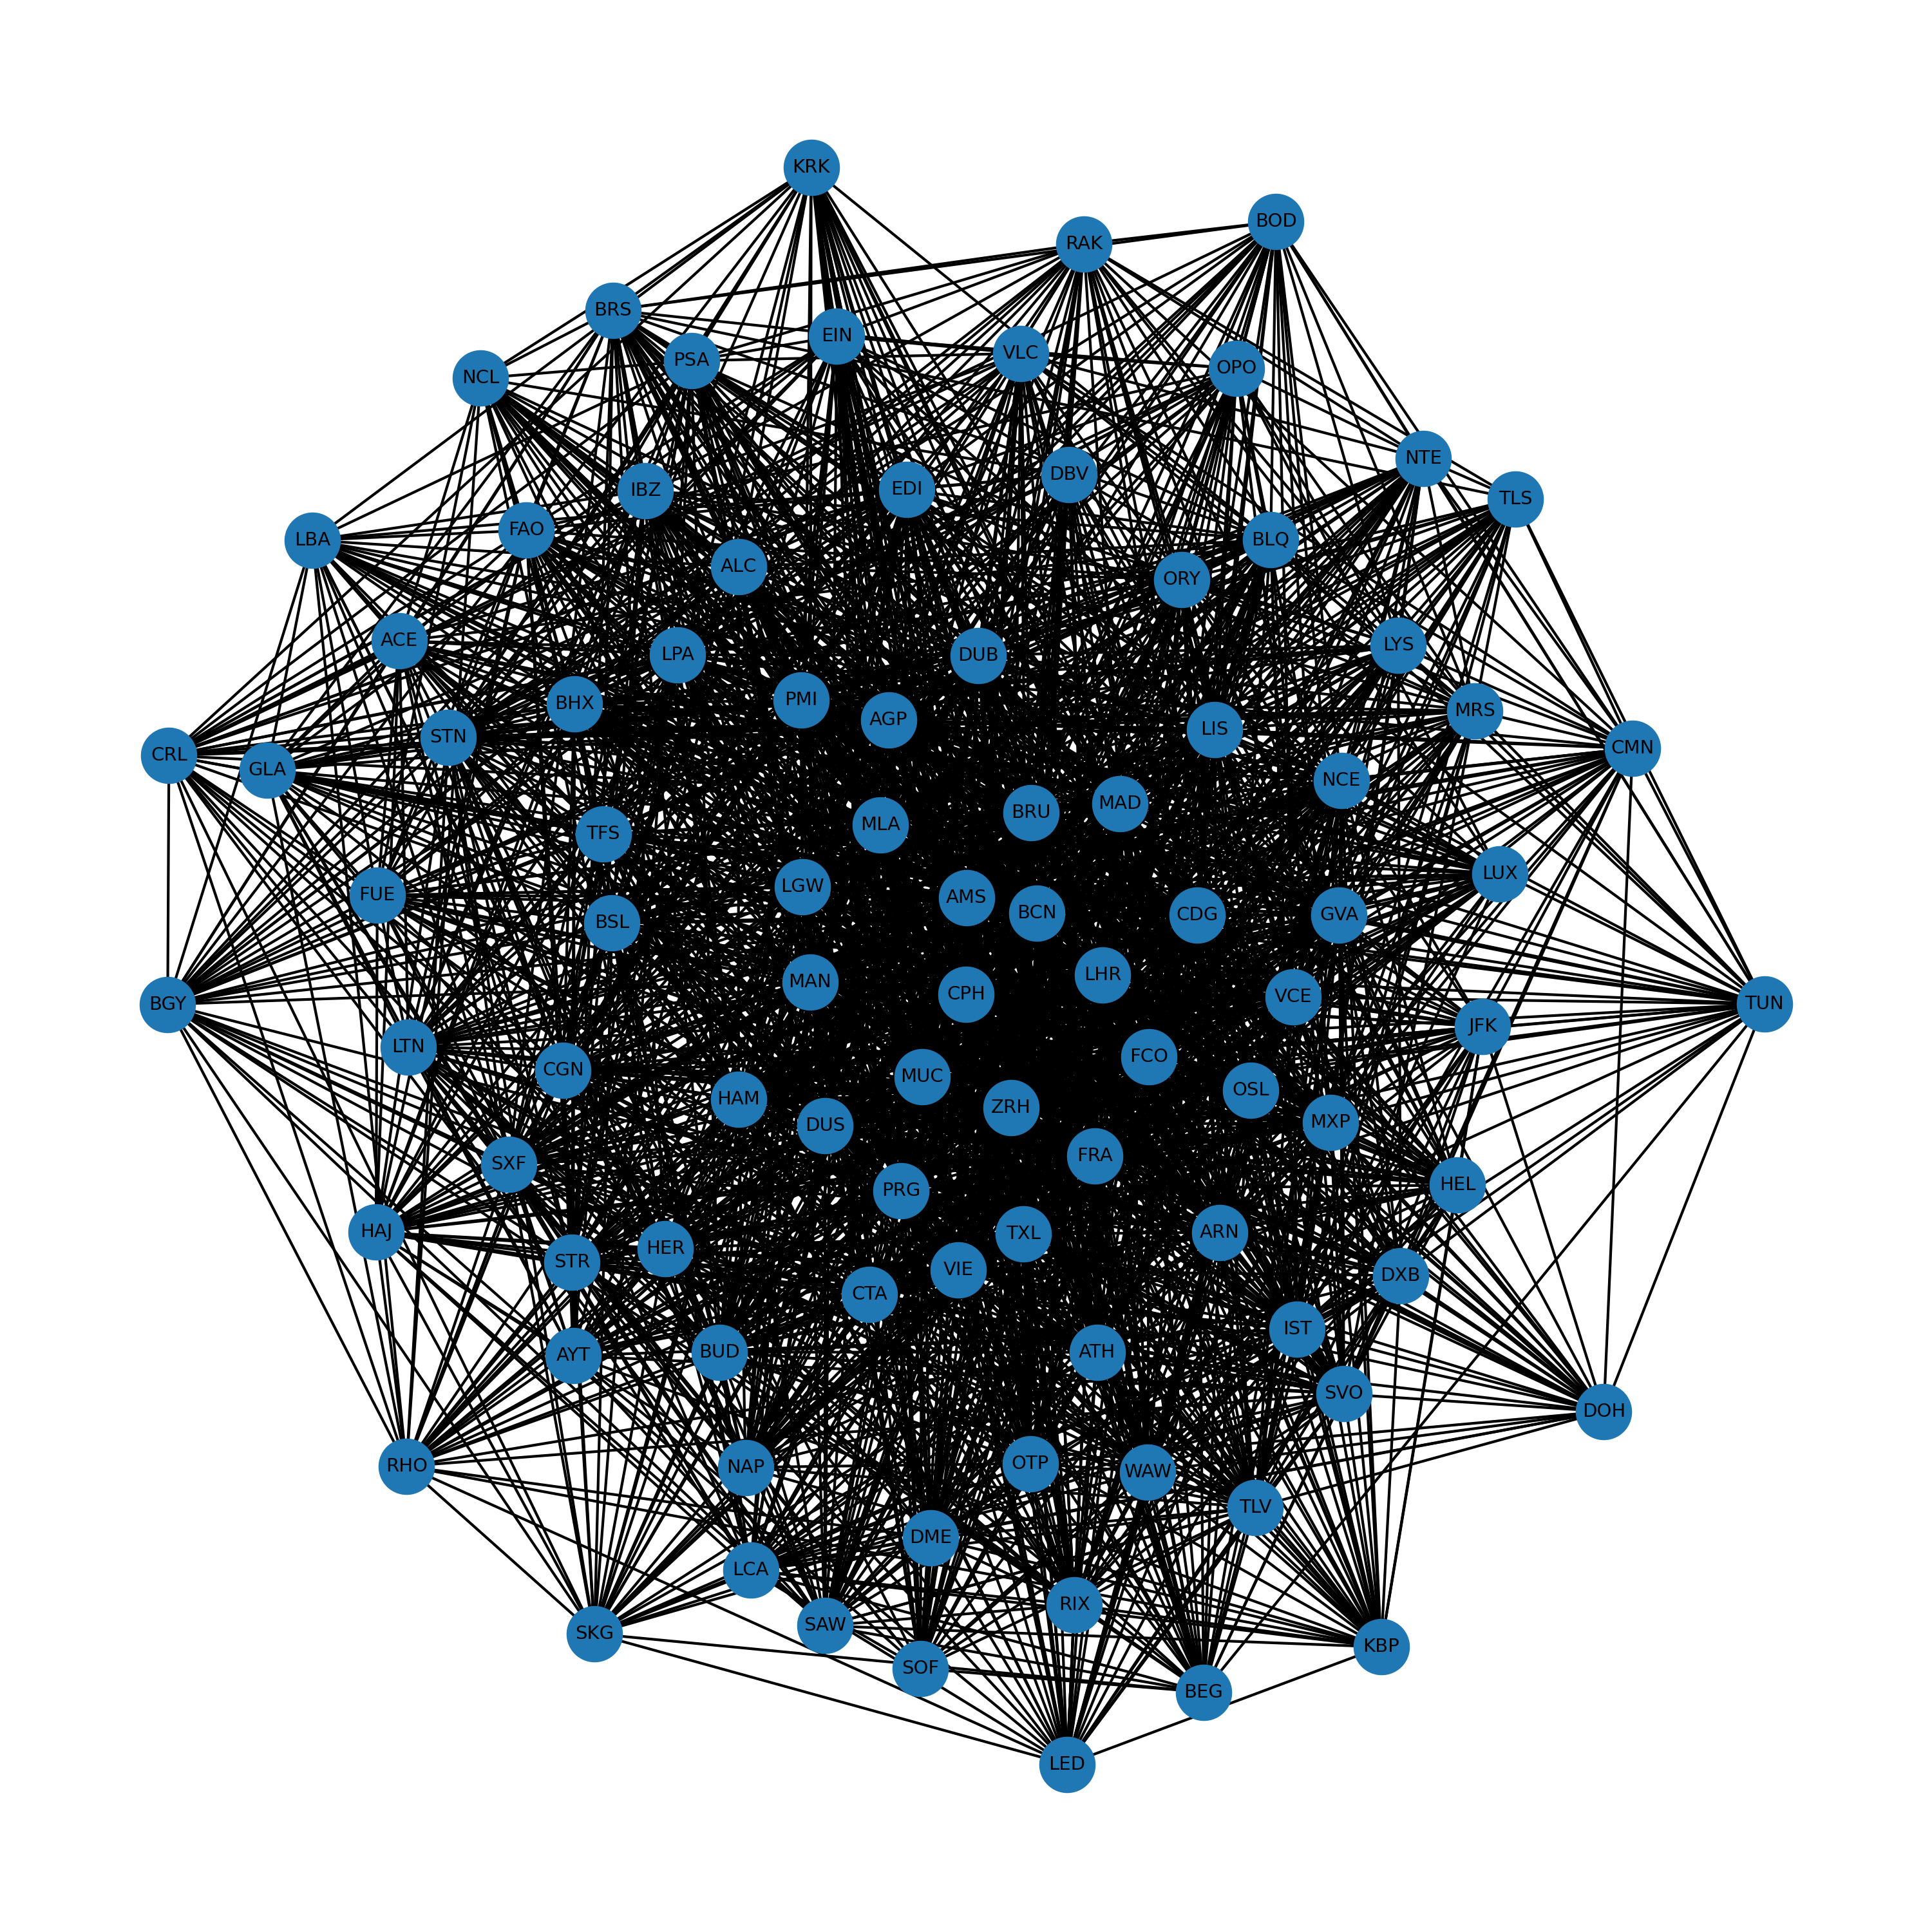
\includegraphics[width=0.9\textwidth]{chapter6/immagini/max_kcore_graph.png}
\caption{Visualizzazione del massimo k-core della rete.}
\label{fig:max_kcore_graph}
\end{figure}

La Figura~\ref{fig:max_kcore_graph} mostra con evidenza un sottografo estremamente denso, nel quale quasi tutti i nodi risultano fortemente intrecciati tra loro. Questa visualizzazione conferma in modo intuitivo il significato del massimo core number osservato e rafforza l’interpretazione del massimo k-core come cuore strutturale della rete.

\section{Ego-network di aeroporti centrali}

Per analizzare la struttura locale delle connessioni è stato effettuato lo studio di due ego-network, centrate rispettivamente sugli aeroporti FRA e DXB. La scelta di questi nodi è stata motivata dai risultati emersi nei capitoli precedenti: FRA risulta particolarmente rilevante nei ranking di degree e closeness, mentre DXB compare con forza sia nella betweenness sia nella closeness.

L’ego-network di un nodo comprende il nodo stesso, tutti i suoi vicini diretti e le connessioni presenti tra essi. In questo modo è possibile osservare non soltanto l’ampiezza del vicinato di un aeroporto, ma anche il livello di coesione locale che lo caratterizza.

\begin{figure}[H]
\centering
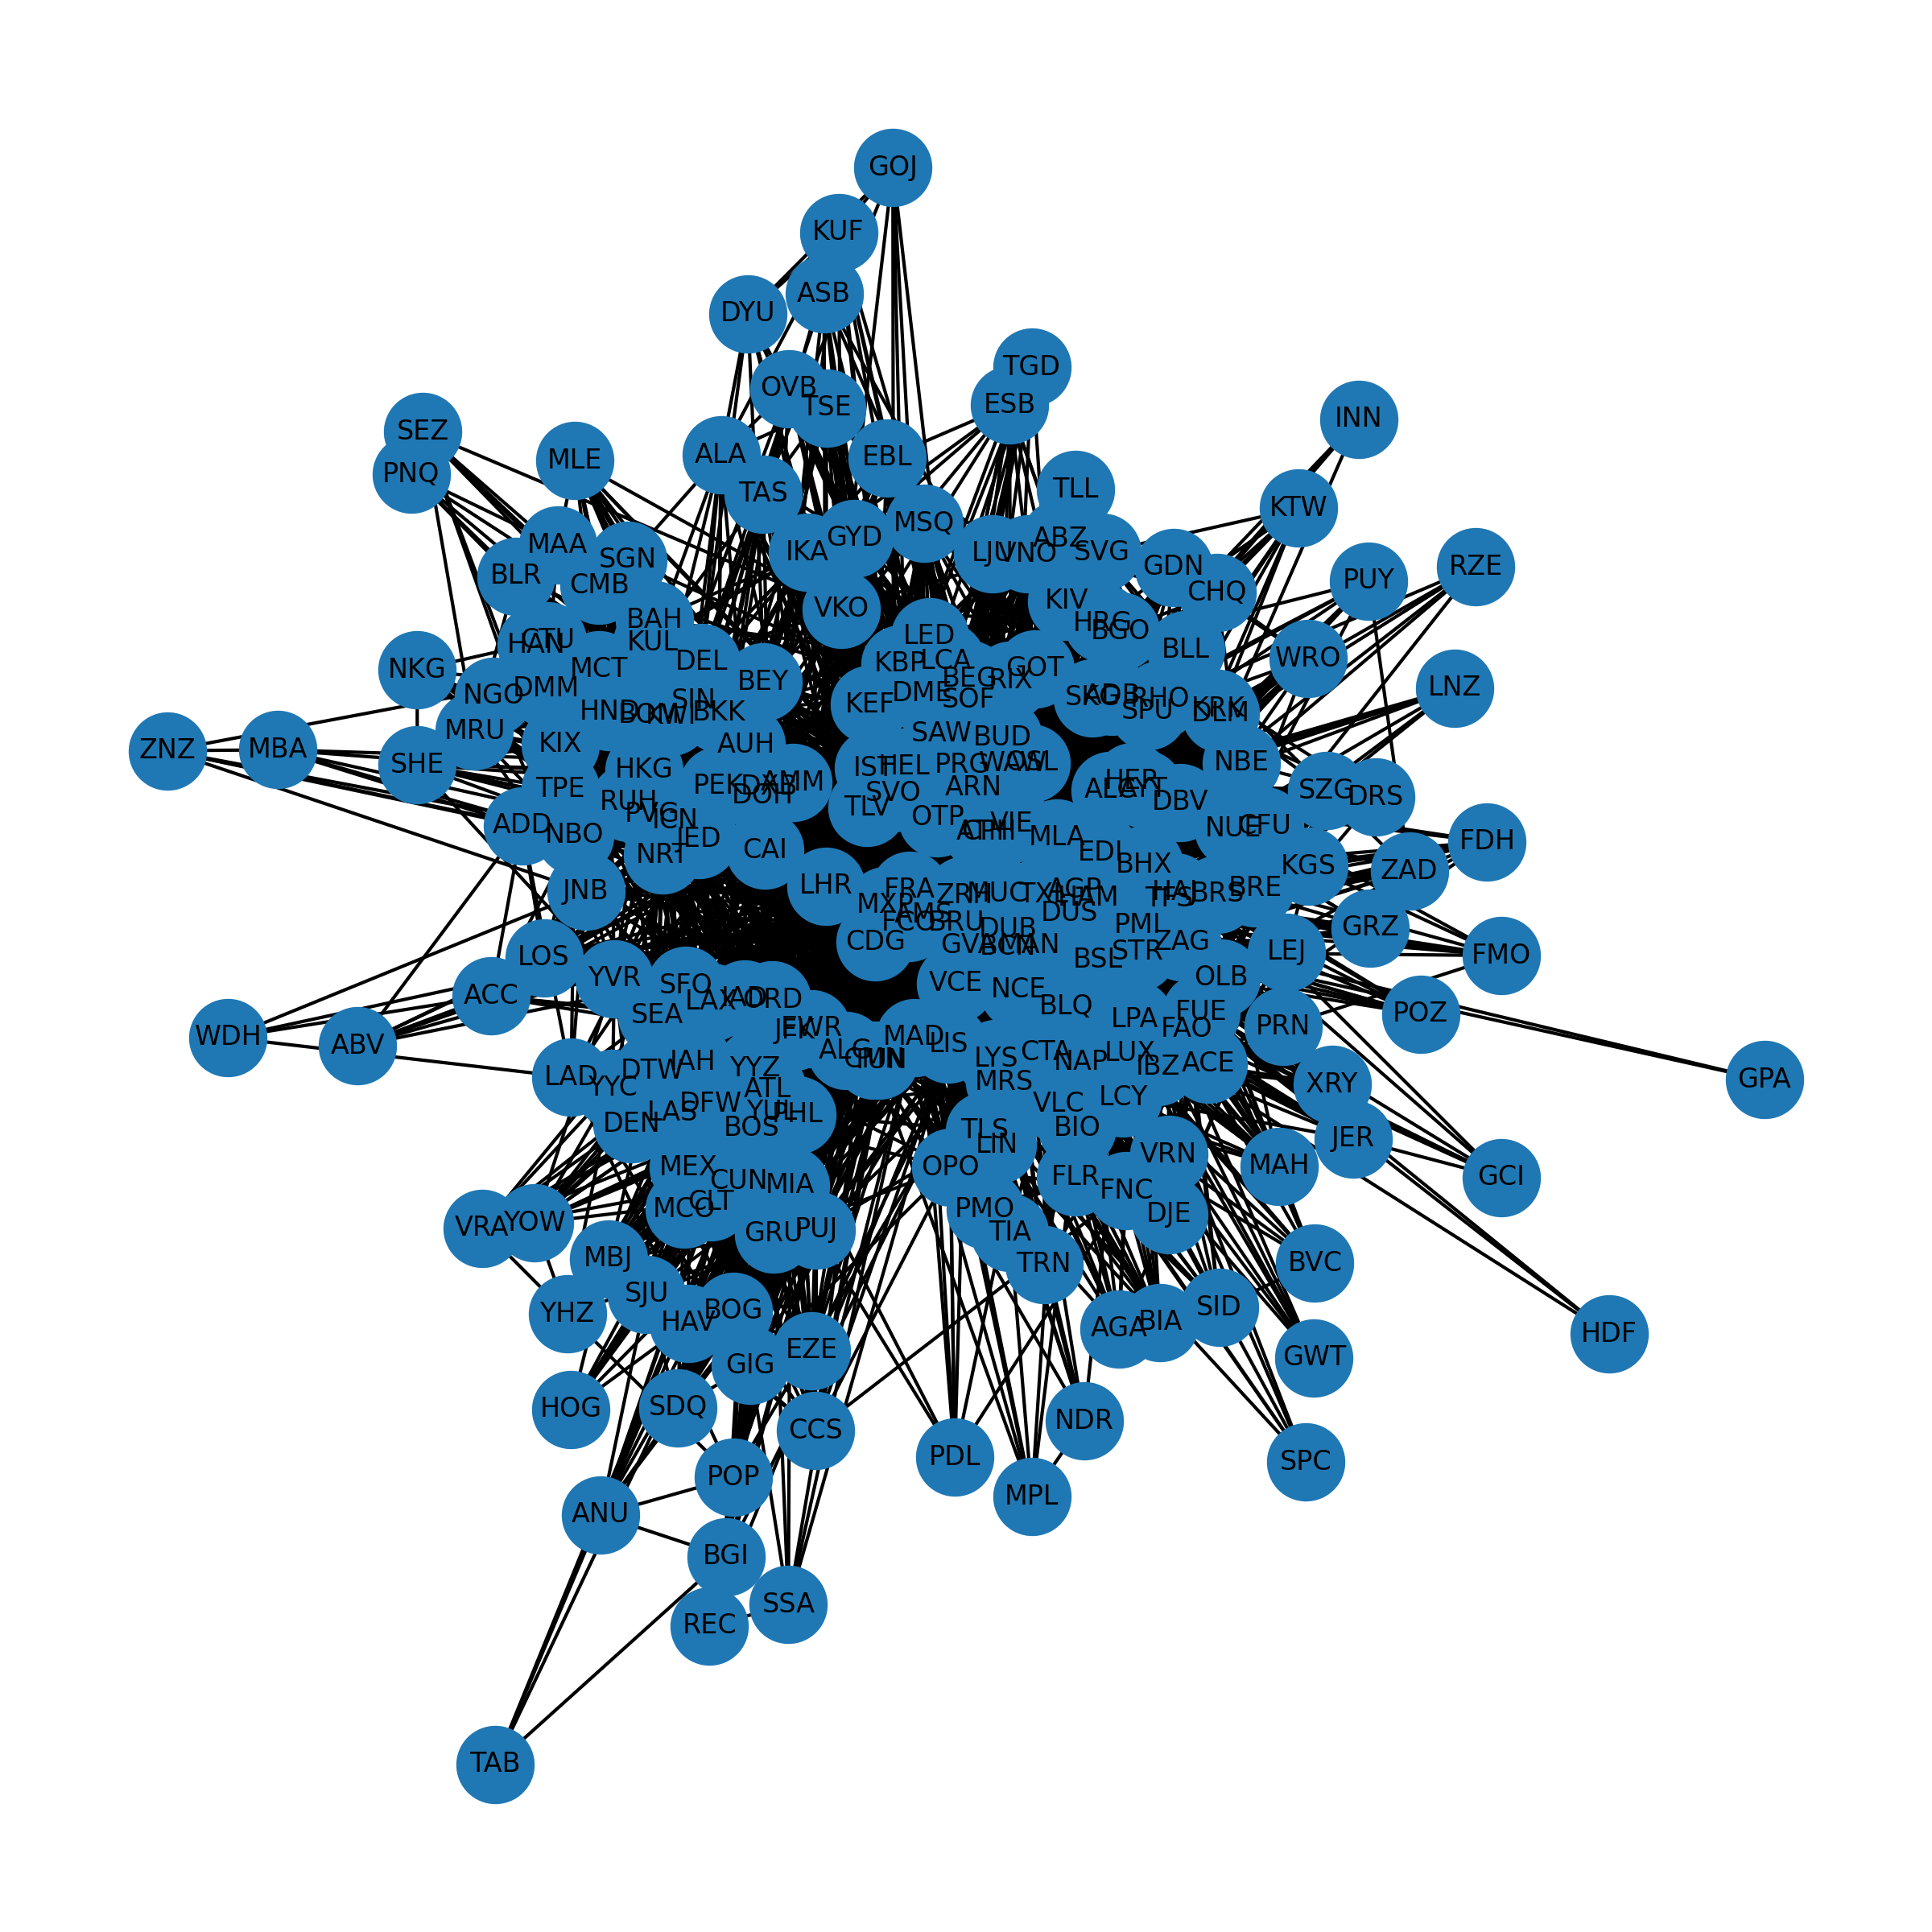
\includegraphics[width=0.9\textwidth]{chapter6/immagini/ego_network_FRA.png}
\caption{Ego-network dell’aeroporto FRA.}
\label{fig:ego_fra}
\end{figure}

\begin{figure}[H]
\centering
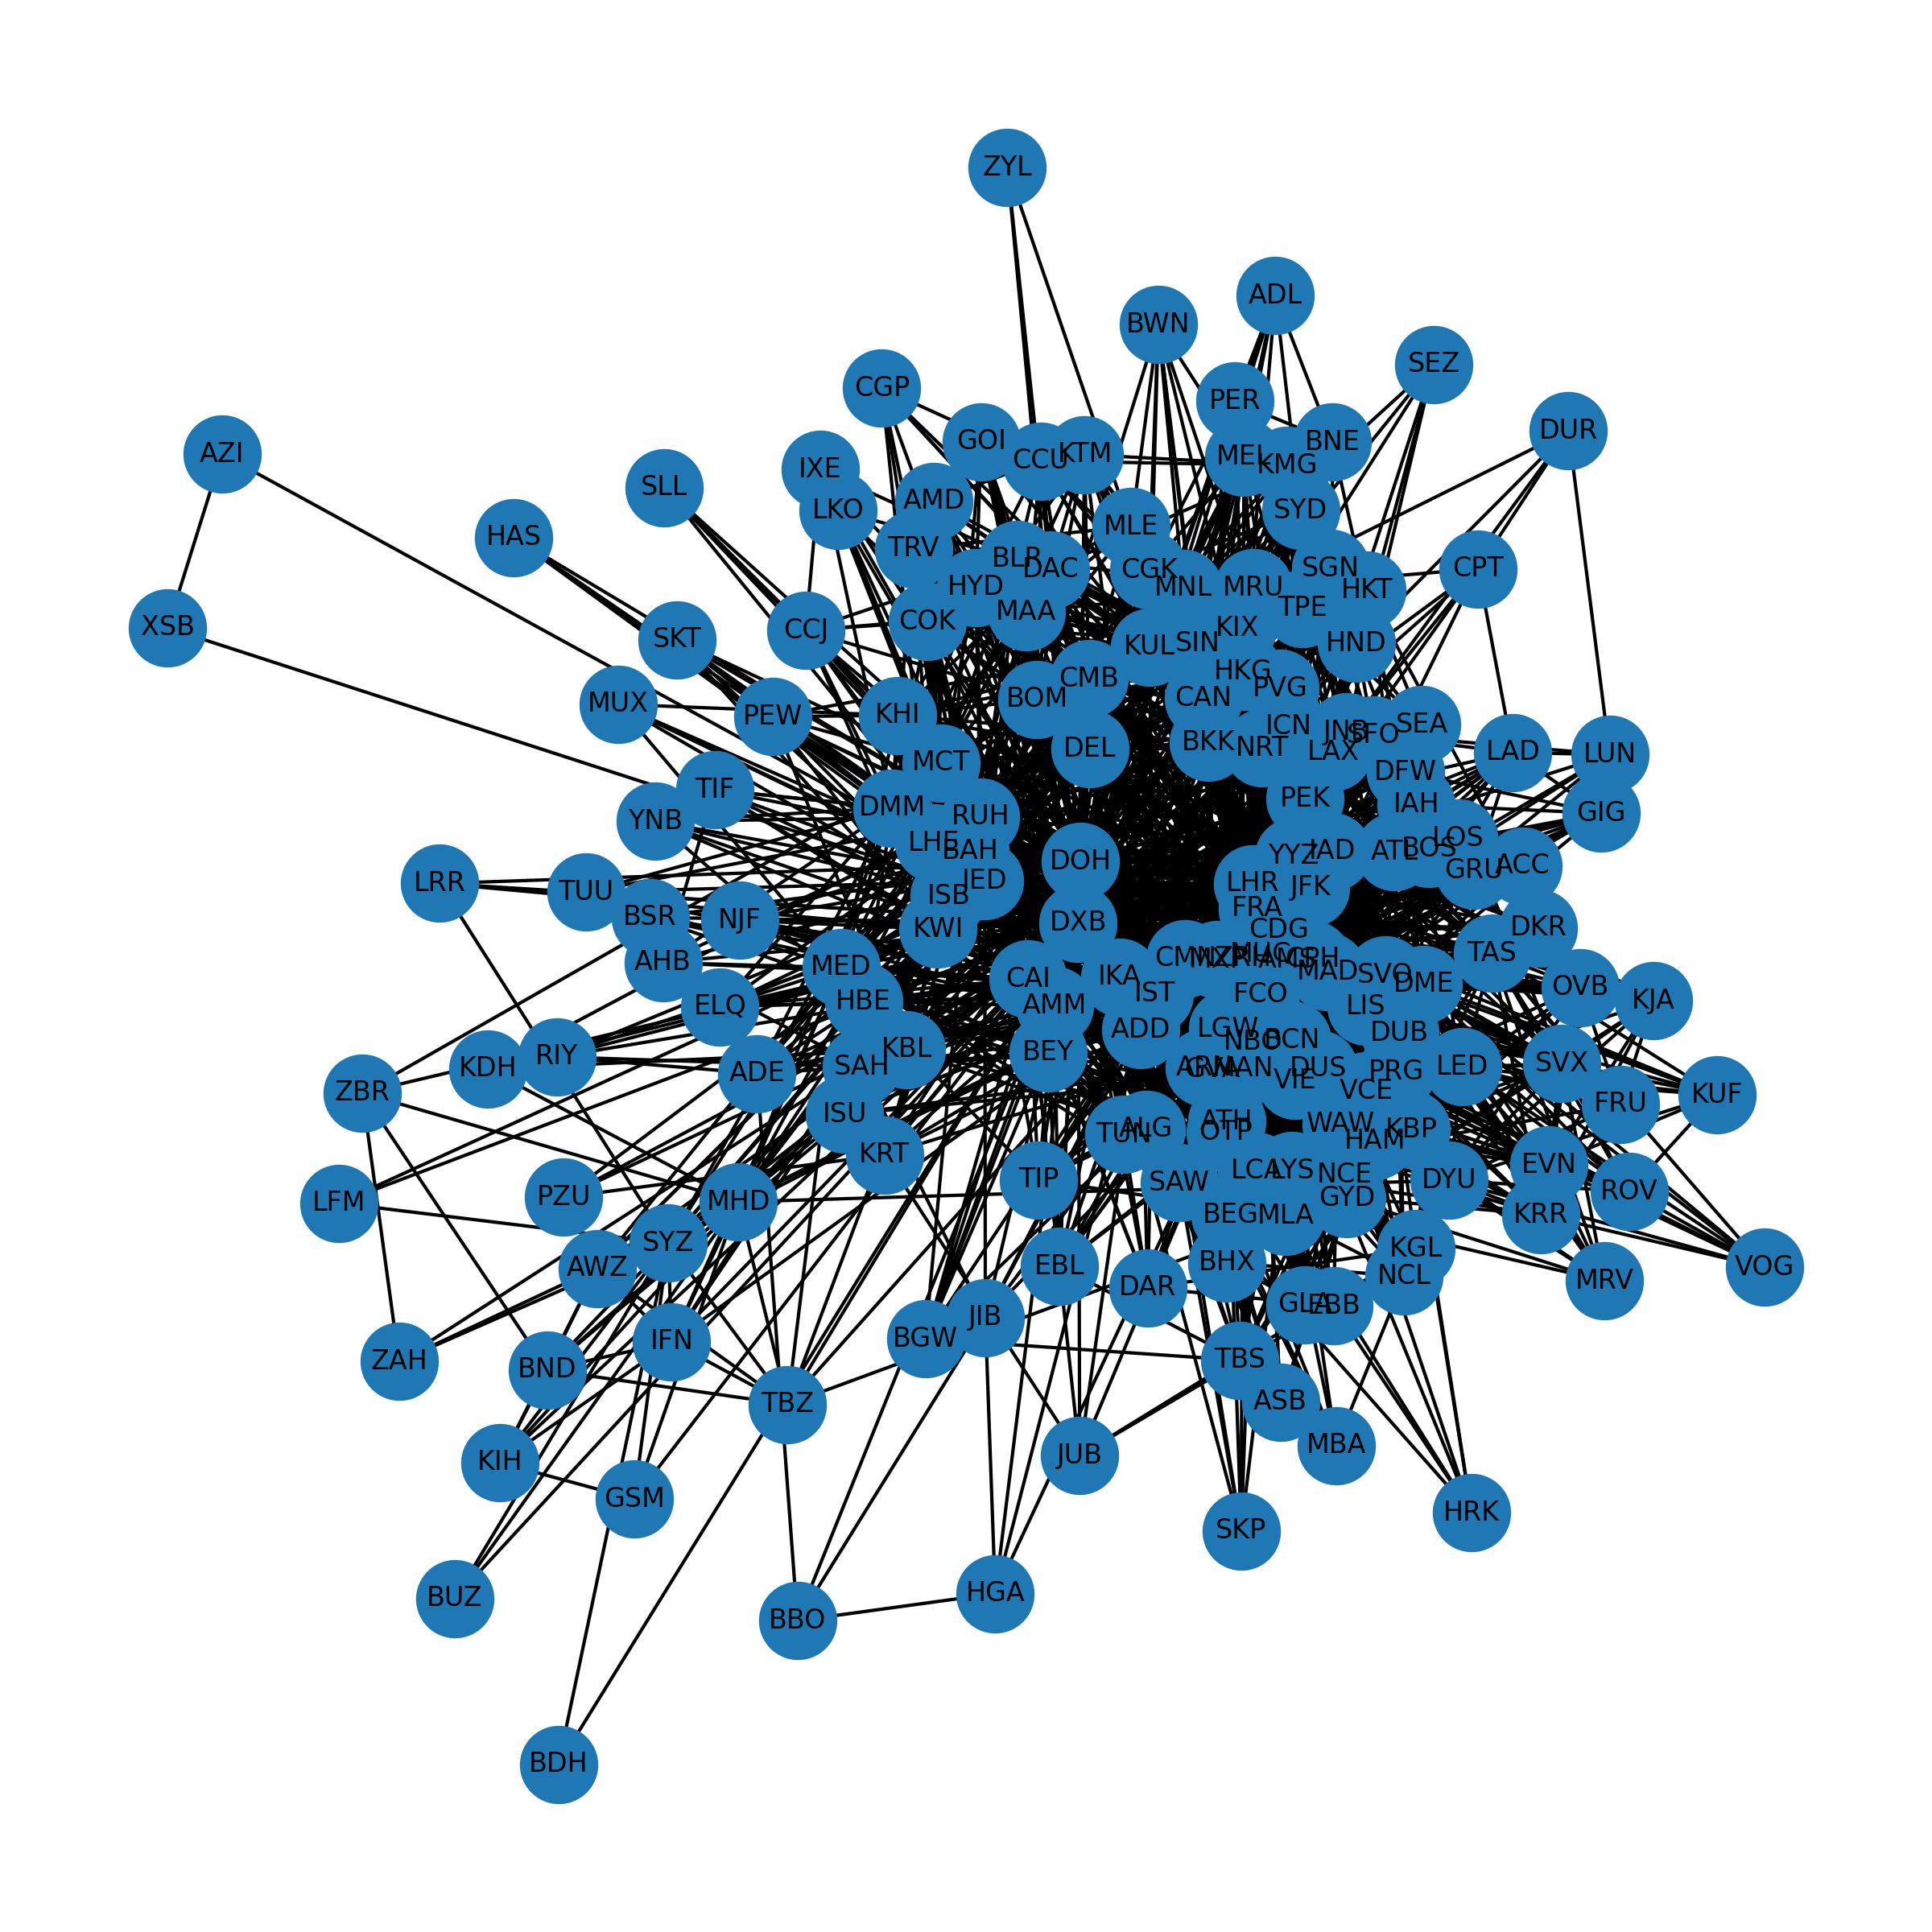
\includegraphics[width=0.9\textwidth]{chapter6/immagini/ego_network_DXB.png}
\caption{Ego-network dell’aeroporto DXB.}
\label{fig:ego_dxb}
\end{figure}

Nel caso di FRA, l’ego-network contiene 245 nodi e 4601 archi, con un grado nel grafo principale pari a 244. L’ego-network di DXB risulta invece composta da 189 nodi e 2613 archi, con grado pari a 188. Questi valori confermano il ruolo centrale di entrambi gli aeroporti, pur mostrando una maggiore ampiezza e densità locale nel caso di FRA.

Dal punto di vista interpretativo, FRA appare come un hub europeo con una rete locale molto estesa e fortemente intrecciata, mentre DXB mostra una struttura leggermente più contenuta ma comunque altamente centrale e strategica, coerente con il suo ruolo di snodo intercontinentale.

Per migliorare la leggibilità delle ego-network, sono state prodotte anche due versioni alternative in cui il nodo centrale viene evidenziato in modo più netto rispetto ai nodi periferici.

\begin{figure}[H]
\centering
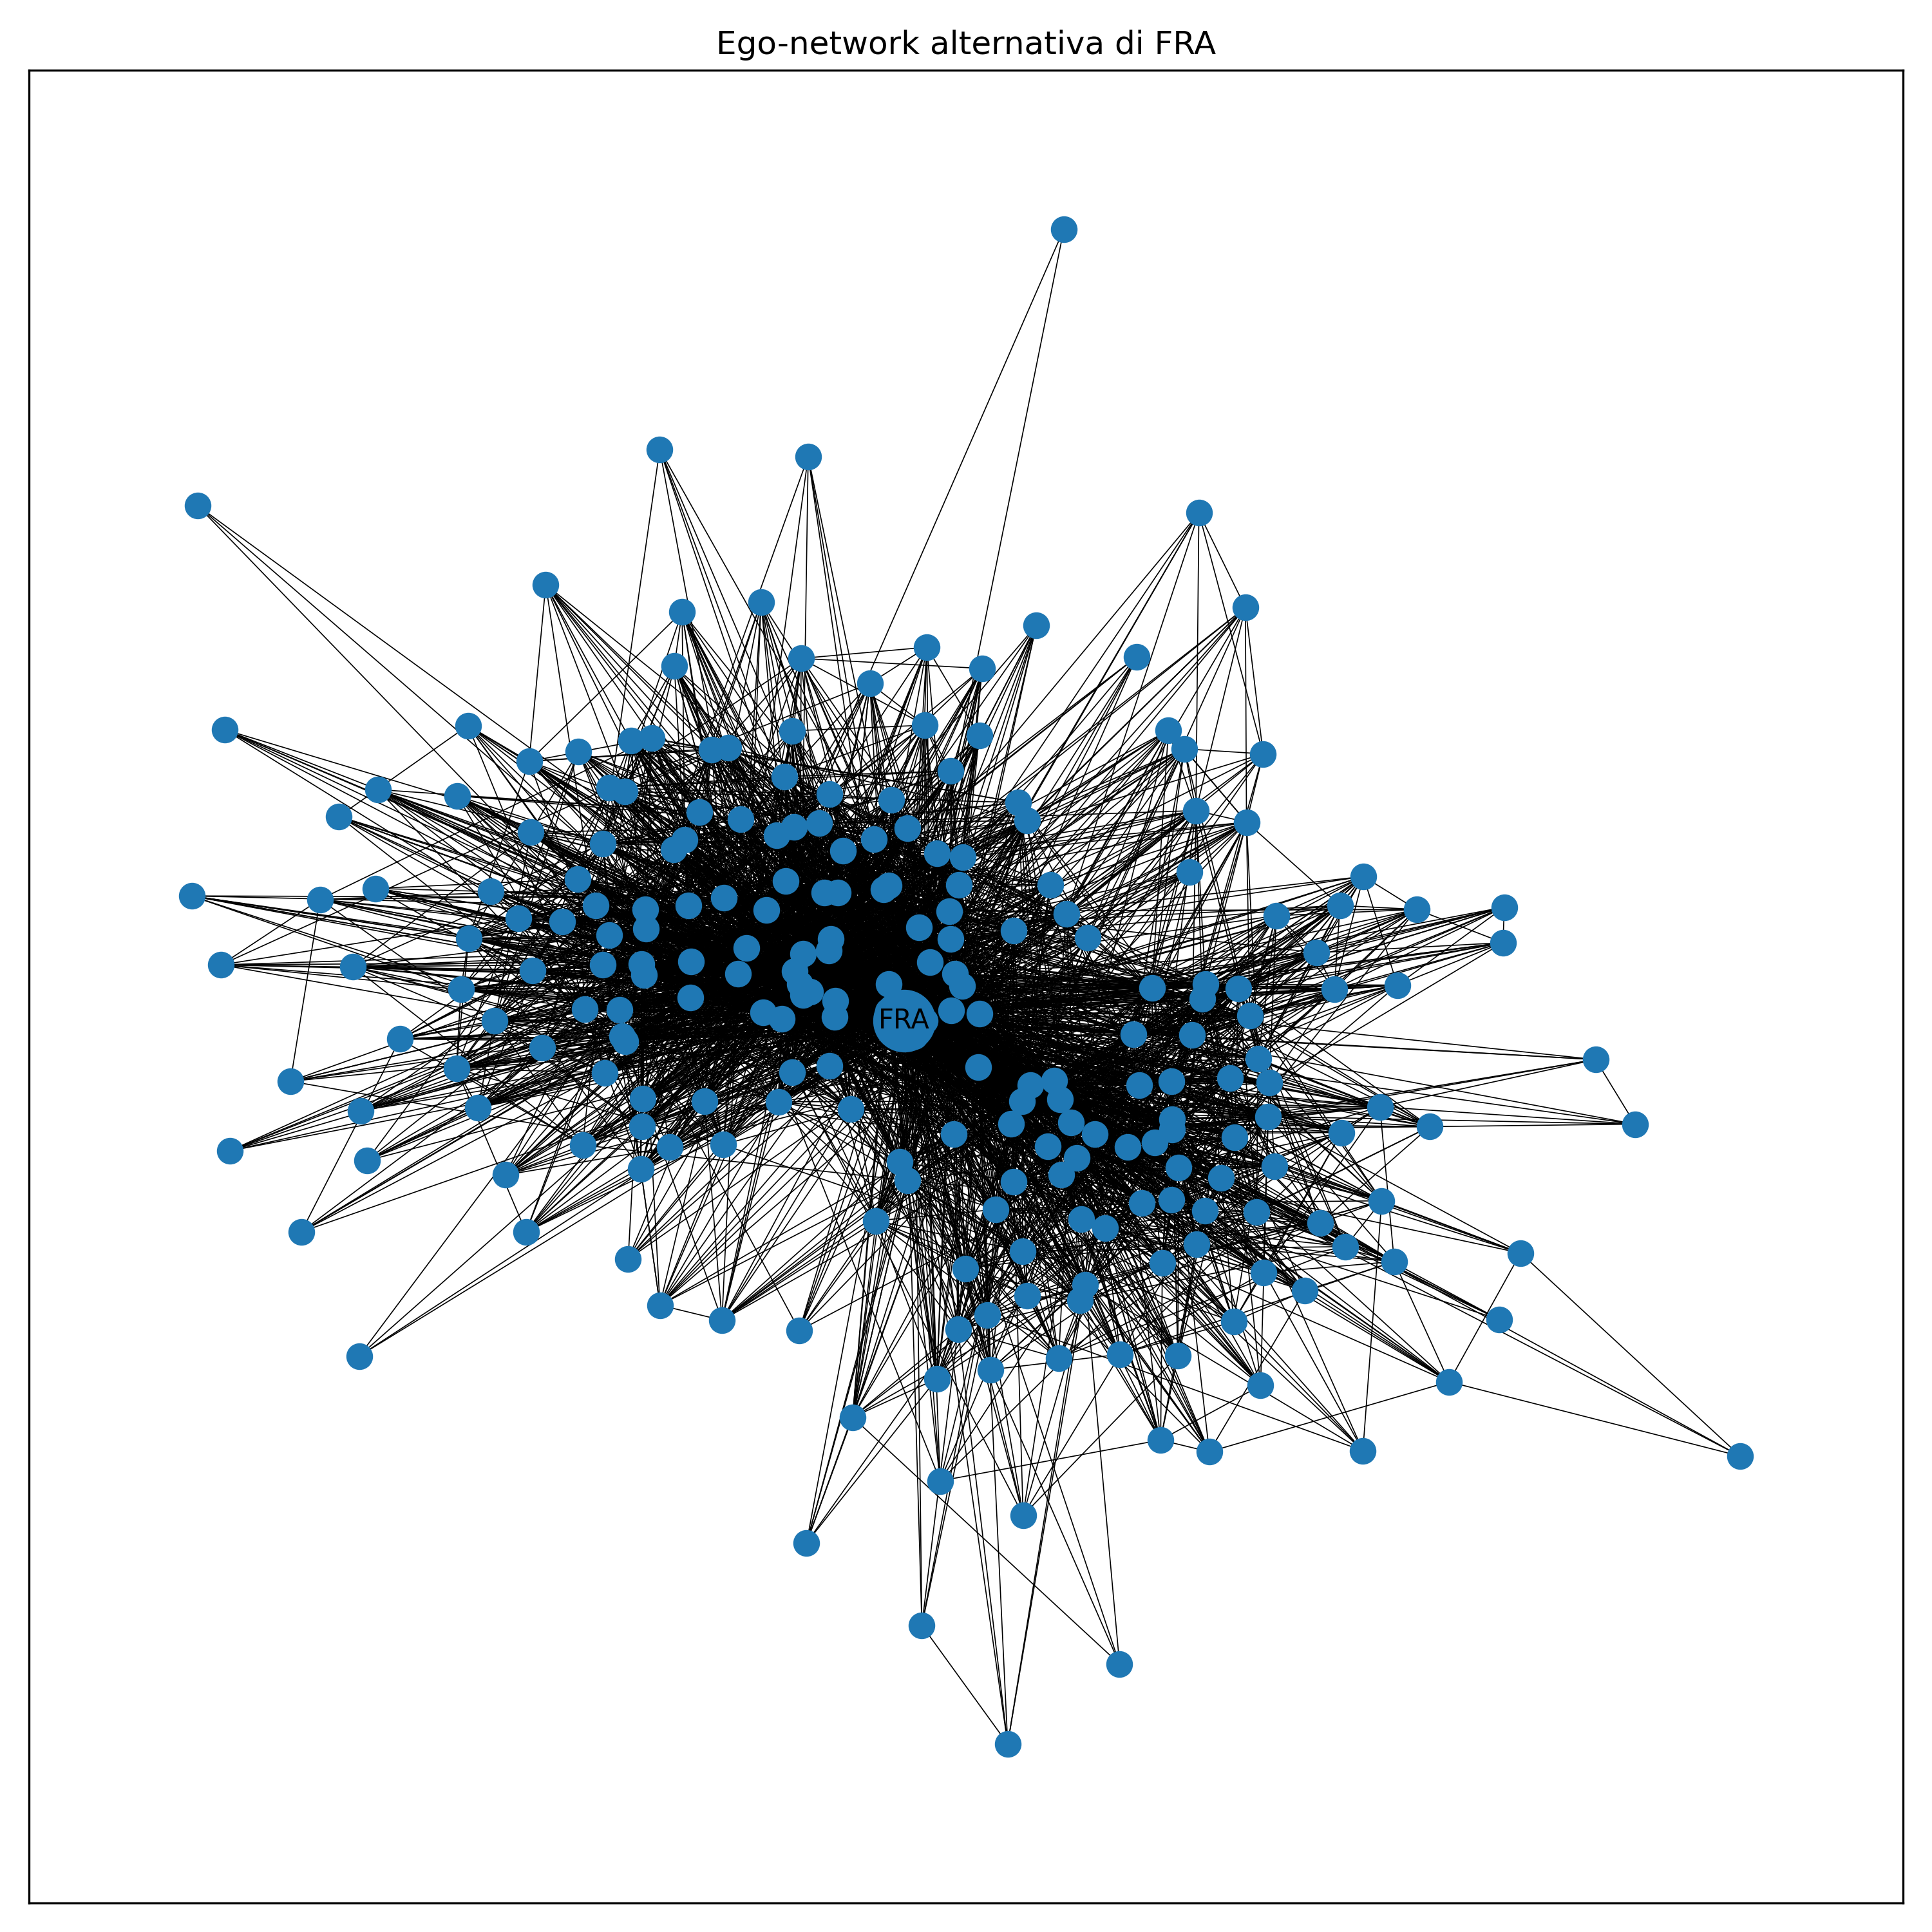
\includegraphics[width=0.9\textwidth]{chapter6/immagini/ego_network_FRA_alt.png}
\caption{Versione alternativa dell’ego-network di FRA con nodo centrale evidenziato.}
\label{fig:ego_fra_alt}
\end{figure}

\begin{figure}[H]
\centering
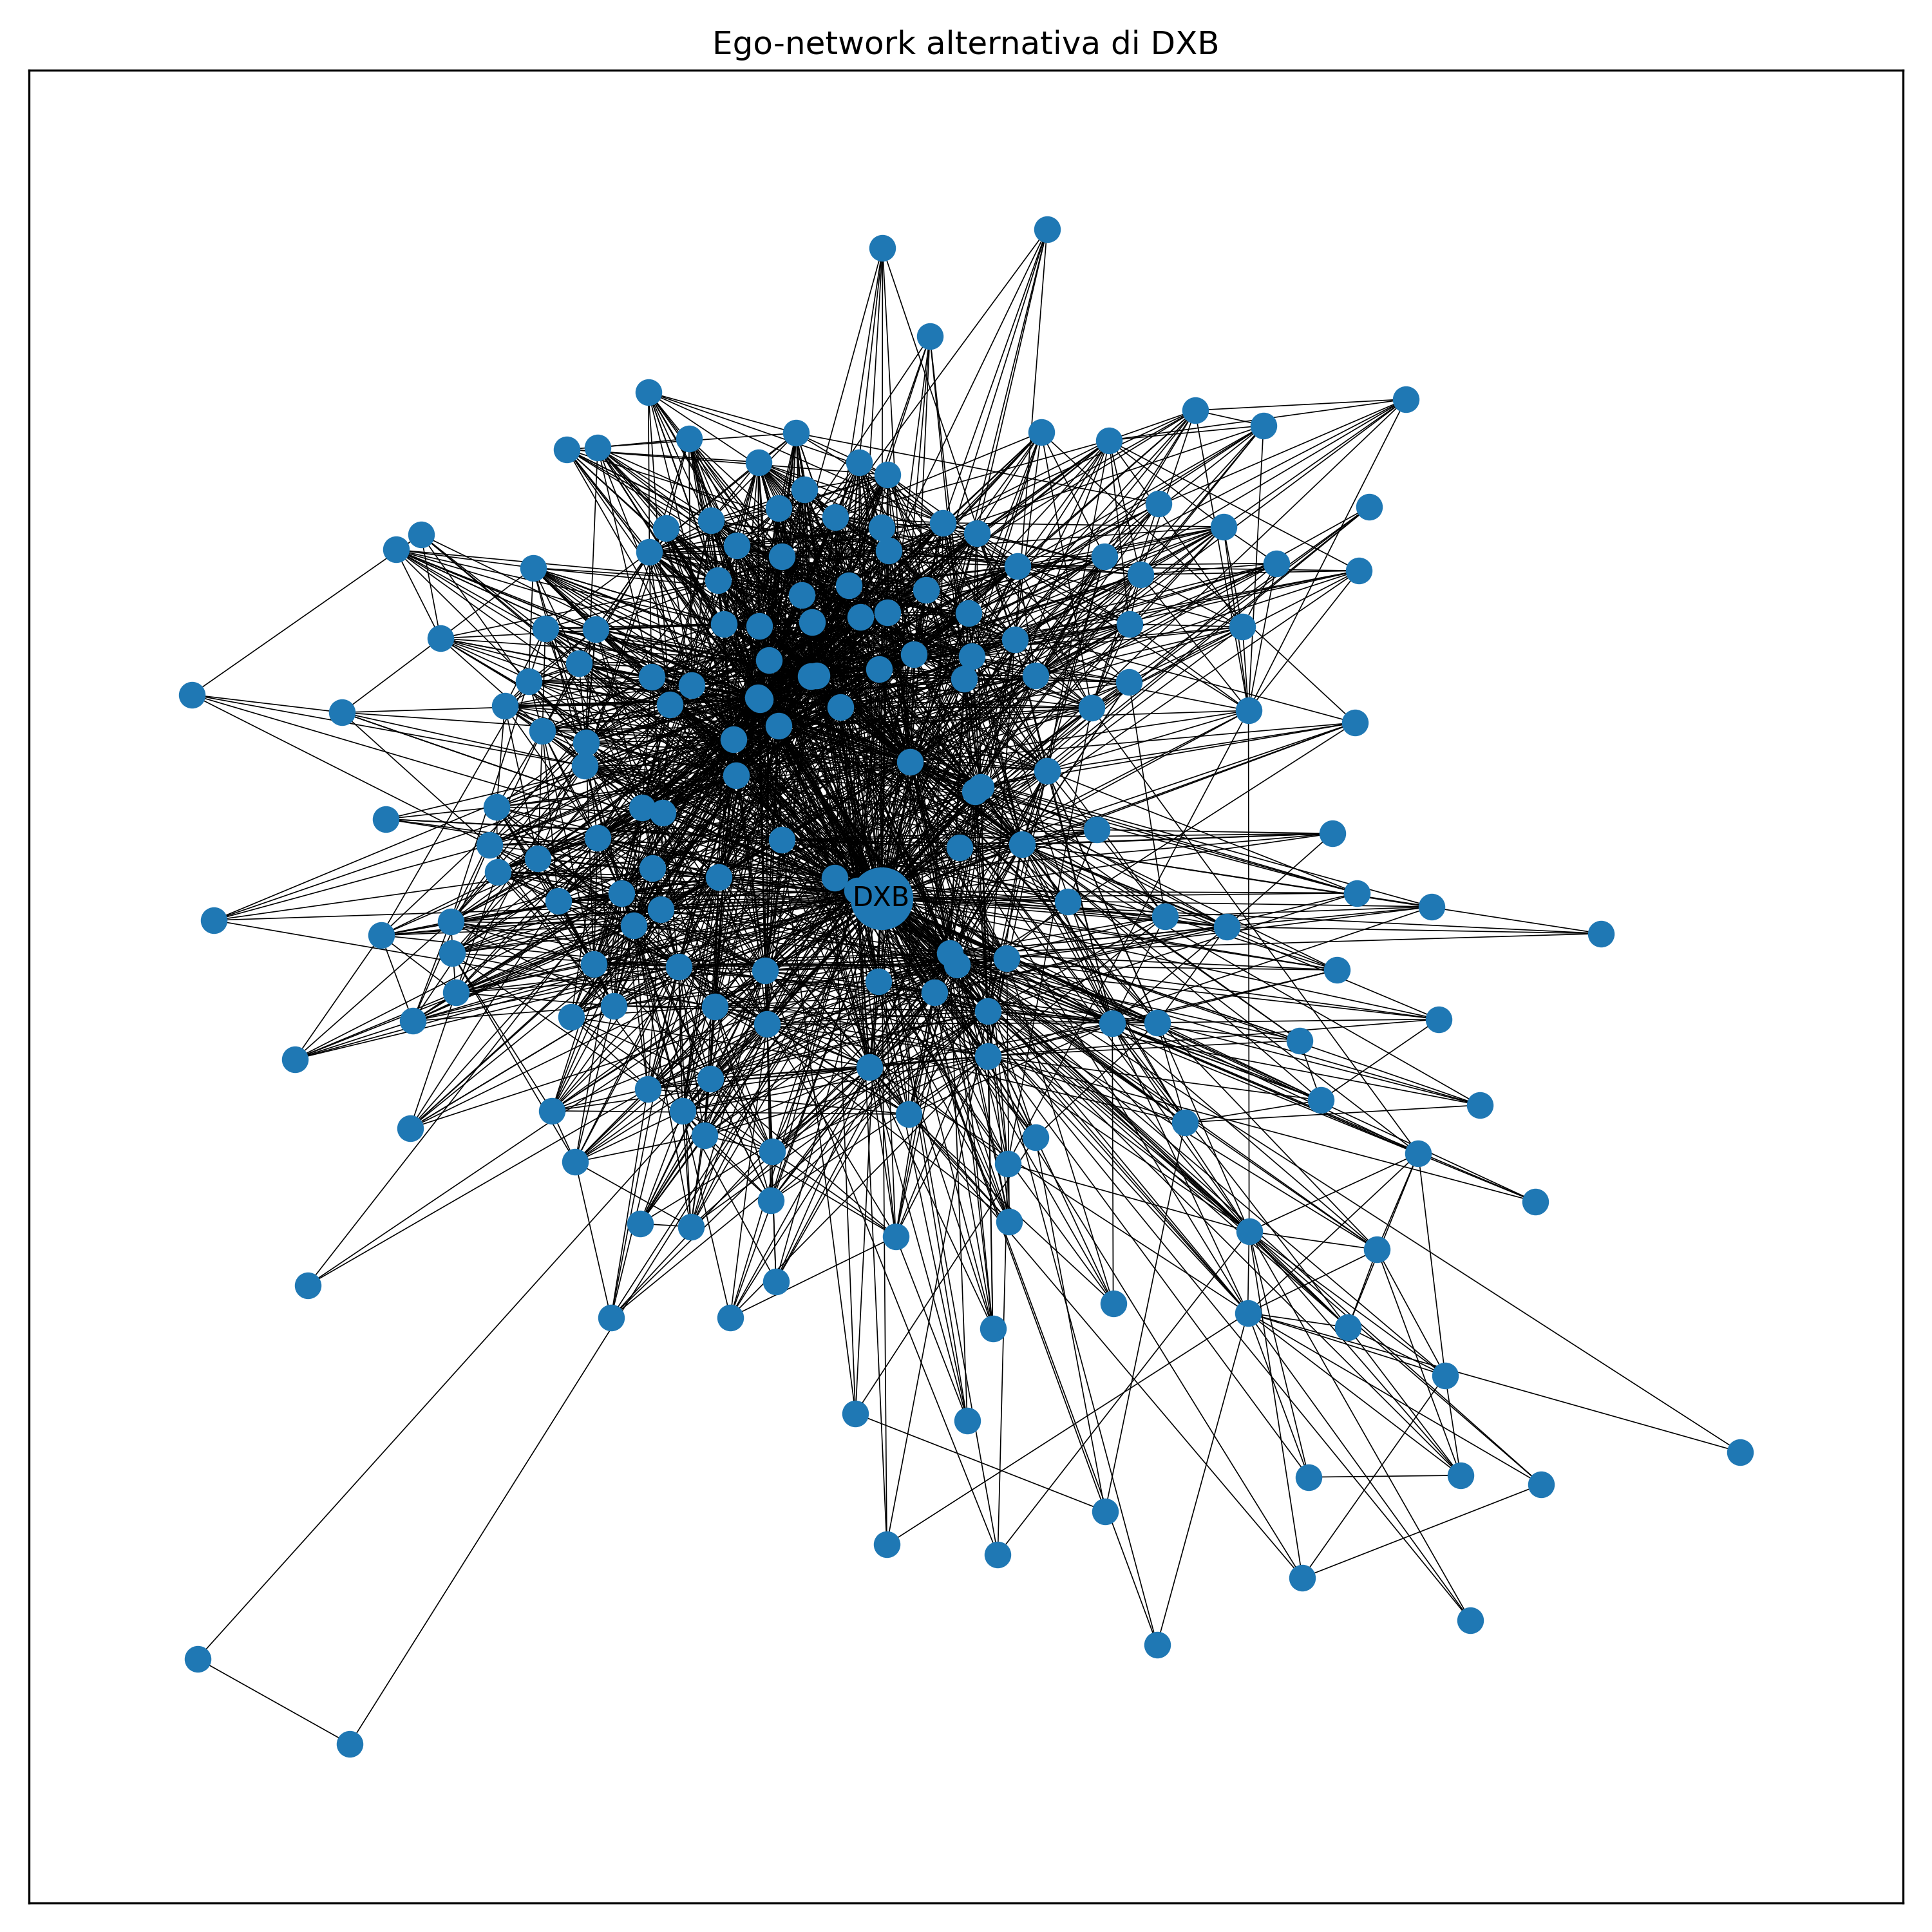
\includegraphics[width=0.9\textwidth]{chapter6/immagini/ego_network_DXB_alt.png}
\caption{Versione alternativa dell’ego-network di DXB con nodo centrale evidenziato.}
\label{fig:ego_dxb_alt}
\end{figure}

Le Figure~\ref{fig:ego_fra_alt} e~\ref{fig:ego_dxb_alt} rendono più immediata l’individuazione del nodo ego e facilitano la lettura della struttura locale. In particolare, si osserva come il vicinato di FRA risulti più ampio e ramificato, mentre quello di DXB appare leggermente più compatto, pur mantenendo un elevato numero di connessioni trasversali.

\section{Clustering coefficient e coesione locale}

Per quantificare in modo più preciso il livello di coesione locale della rete è stato calcolato il \textit{clustering coefficient}.. Questa misura esprime, per ciascun nodo, quanto i suoi vicini tendano a essere collegati tra loro. In una rete di trasporto, un clustering coefficient elevato indica quindi che un aeroporto appartiene a un contesto locale fortemente interconnesso.

\begin{table}[H]
\centering
\caption{Sintesi dei principali risultati relativi al clustering coefficient.}
\label{tab:clustering_summary}
\begin{tabular}{lc}
\toprule
\textbf{Misura} & \textbf{Valore} \\
\midrule
Clustering coefficient medio del grafo & 0.488336 \\
Clustering coefficient di FRA & 0.146968 \\
Clustering coefficient di DXB & 0.137957 \\
\bottomrule
\end{tabular}
\end{table}

Nel grafo non diretto principale, il clustering coefficient medio risulta pari a 0.488336, valore che indica una tendenza non trascurabile alla formazione di gruppi locali coesi. Accanto a questo valore globale, sono stati considerati anche i valori locali del clustering coefficient per FRA e DXB, già analizzati tramite ego-network, così da collegare la rappresentazione visiva delle loro connessioni con una misura quantitativa di coesione. In particolare, FRA presenta un clustering coefficient pari a 0.146968, mentre DXB assume un valore pari a 0.137957. Questi risultati mostrano che, pur essendo hub molto centrali e molto estesi, i loro vicinati non sono composti da gruppi completamente chiusi, ma mantengono una struttura più aperta e articolata.

Per evitare che nei primi posti del ranking compaiano nodi con pochissimi vicini e quindi valori poco significativi, il confronto tra aeroporti è stato effettuato considerando soltanto i nodi con grado almeno pari a 10.

\begin{figure}[H]
\centering
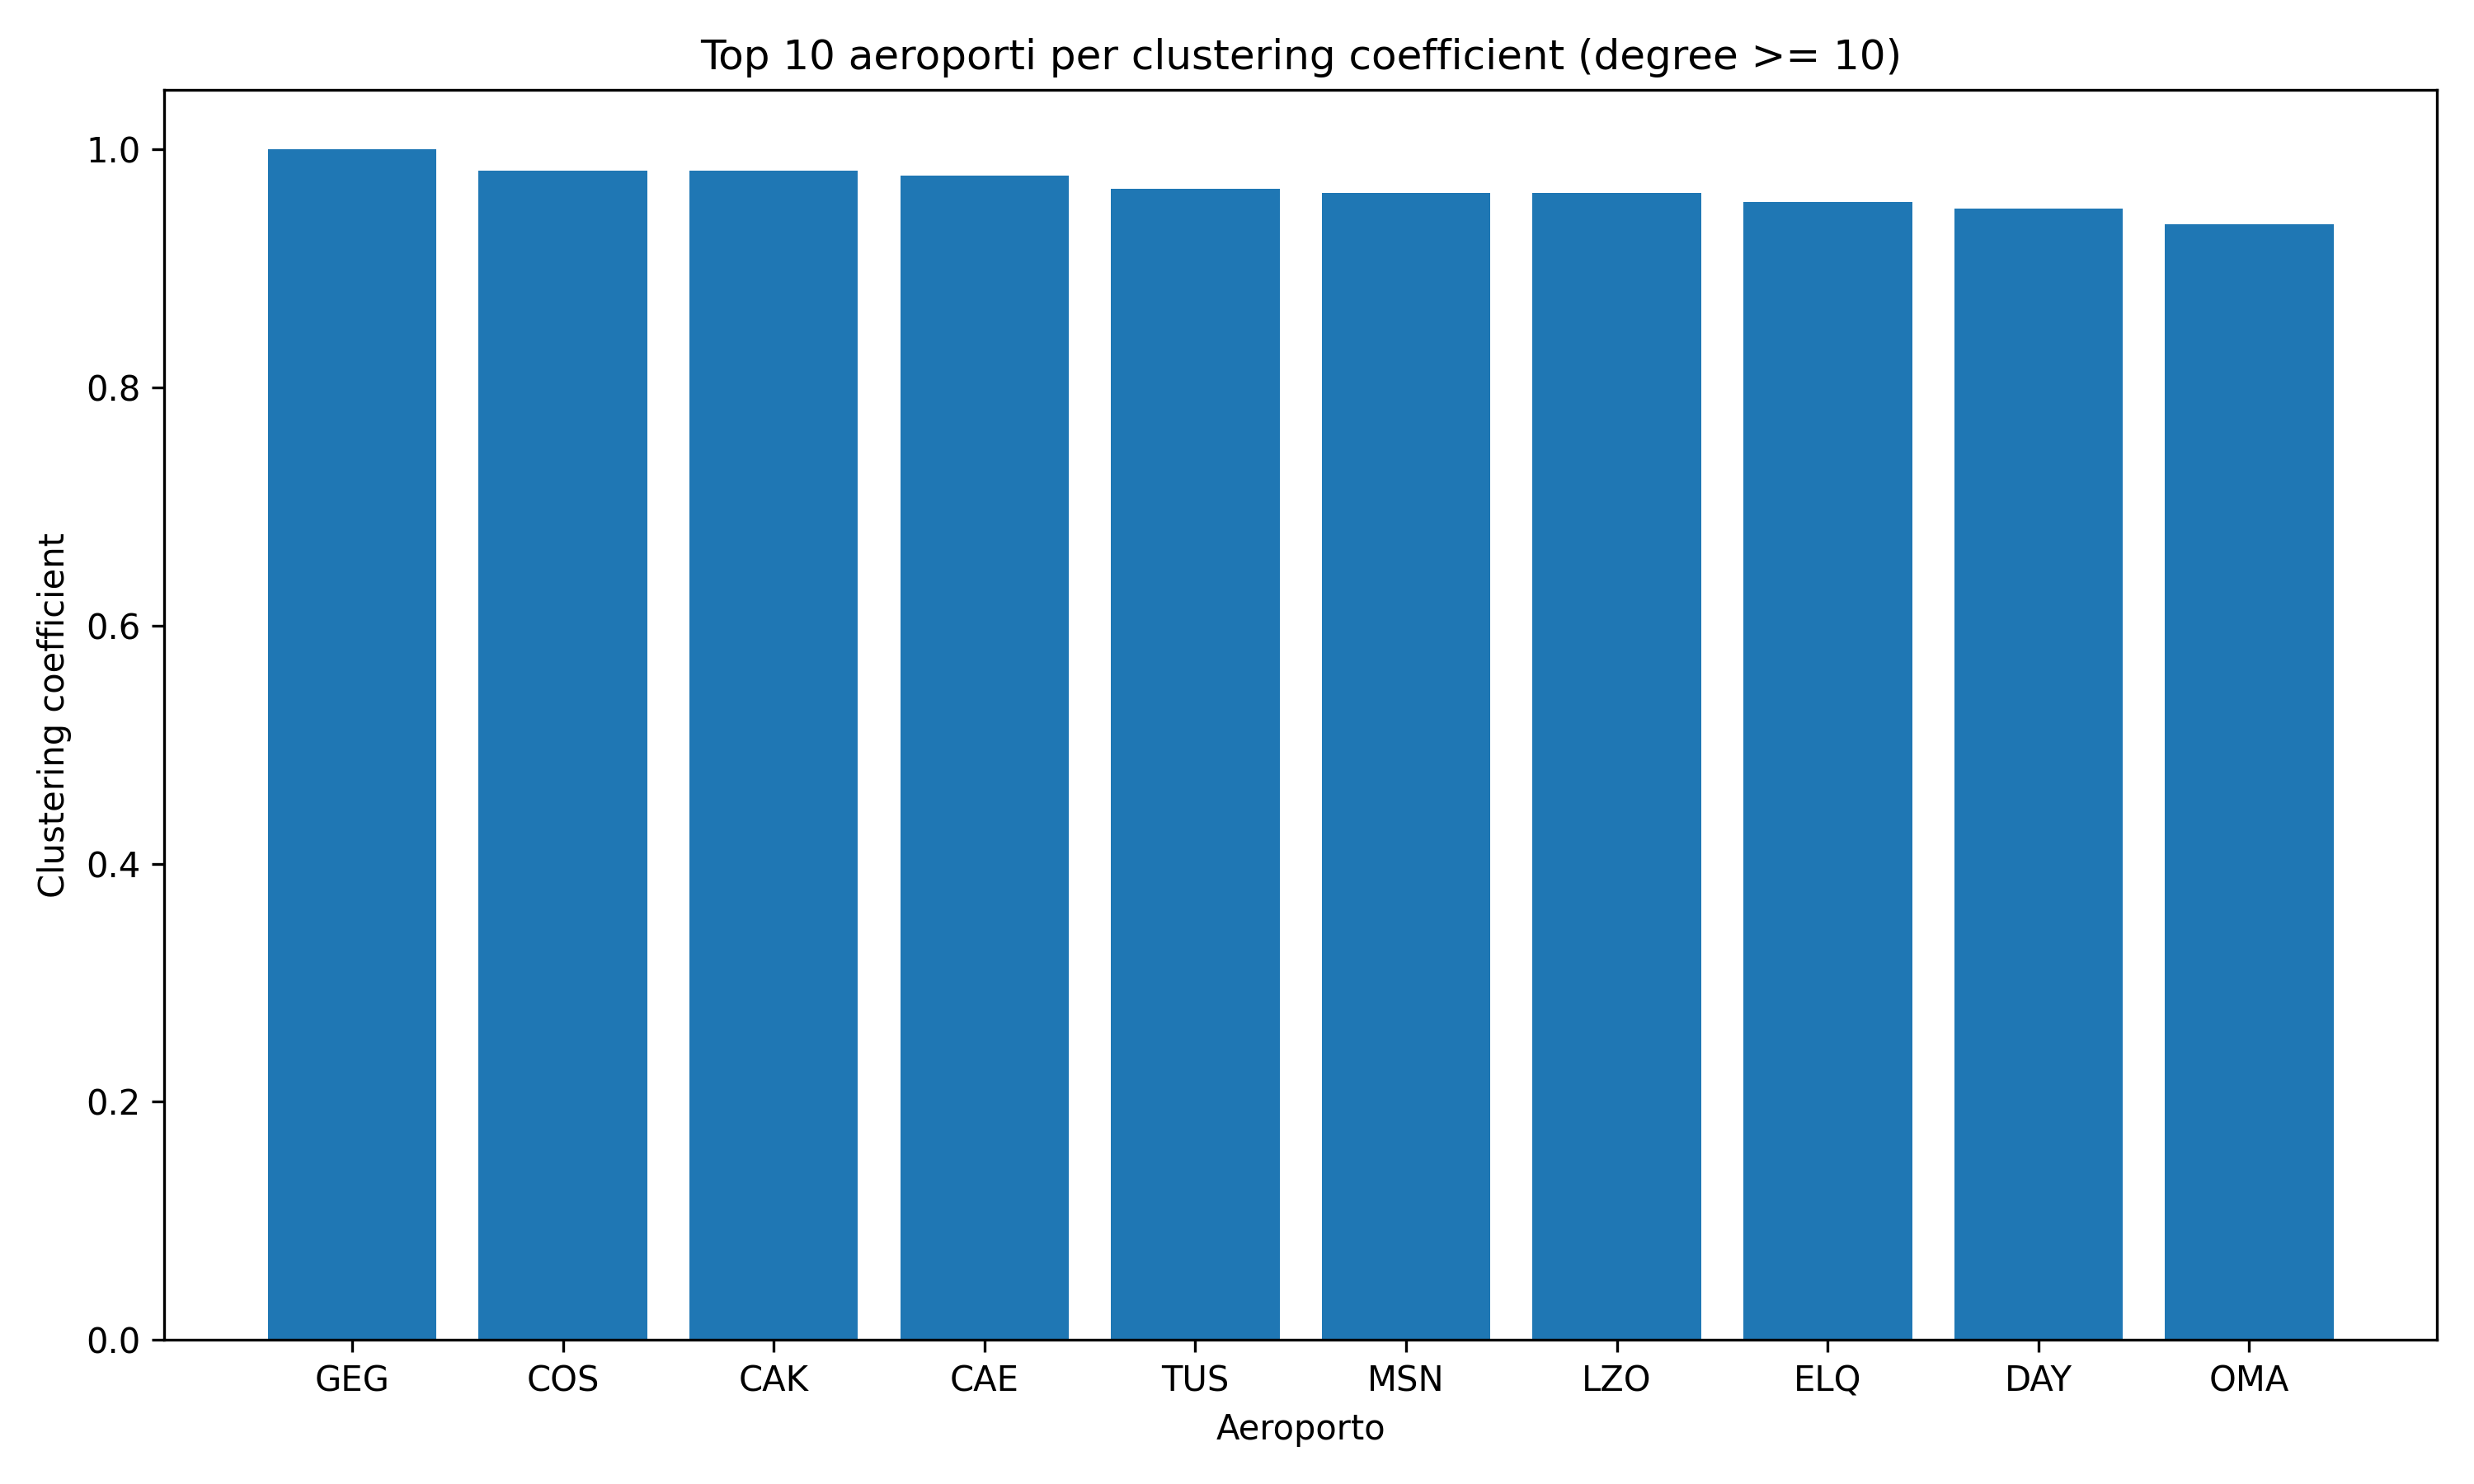
\includegraphics[width=0.9\textwidth]{chapter6/immagini/top10_clustering_coefficient.png}
\caption{Top 10 aeroporti per clustering coefficient, considerando solo nodi con grado $\geq 10$.}
\label{fig:top10_clustering_coefficient}
\end{figure}

La Figura~\ref{fig:top10_clustering_coefficient} mette in evidenza gli aeroporti che risultano inseriti nei contesti locali più coesi della rete. Questo tipo di informazione è complementare rispetto alle centralità globali: un nodo può infatti non essere tra i più influenti dell’intera rete, ma appartenere comunque a una porzione molto compatta e fortemente interconnessa del sistema.

L’analisi del clustering coefficient rafforza quindi l’interpretazione già suggerita dalle ego-network, mostrando che la rete delle rotte aeree non è soltanto organizzata attorno a hub globali, ma presenta anche aree locali caratterizzate da una forte densità di collegamenti reciproci.

\section{Clique massimali}

Per completare l’analisi strutturale è stata effettuata una breve osservazione delle clique massimali presenti nella rete. Una clique è un sottografo completamente connesso, cioè un insieme di nodi in cui ogni coppia di nodi è direttamente collegata. Le clique costituiscono quindi sottostrutture di forte coesione.

Nel grafo analizzato sono state individuate 22763 clique massimali. La dimensione massima osservata è pari a 24 nodi, e risultano presenti 2 clique di dimensione massima. Un esempio di clique massima comprende gli aeroporti MSY, ATL, MCO, CLT, DEN, DTW, MSP, ORD, DFW, IAH, EWR, LAX, LAS, PHL, BOS, PHX, STL, MCI, YYZ, CLE, FLL, SFO, MKE e DCA.

Sebbene questa parte dell’analisi sia stata mantenuta a livello descrittivo, il risultato è comunque significativo, poiché evidenzia la presenza di sottogruppi di aeroporti completamente interconnessi e quindi caratterizzati da un elevato livello di coesione locale.

Per rappresentare in maniera concreta una di queste strutture, è stata anche visualizzata una clique massima.

\begin{figure}[H]
\centering
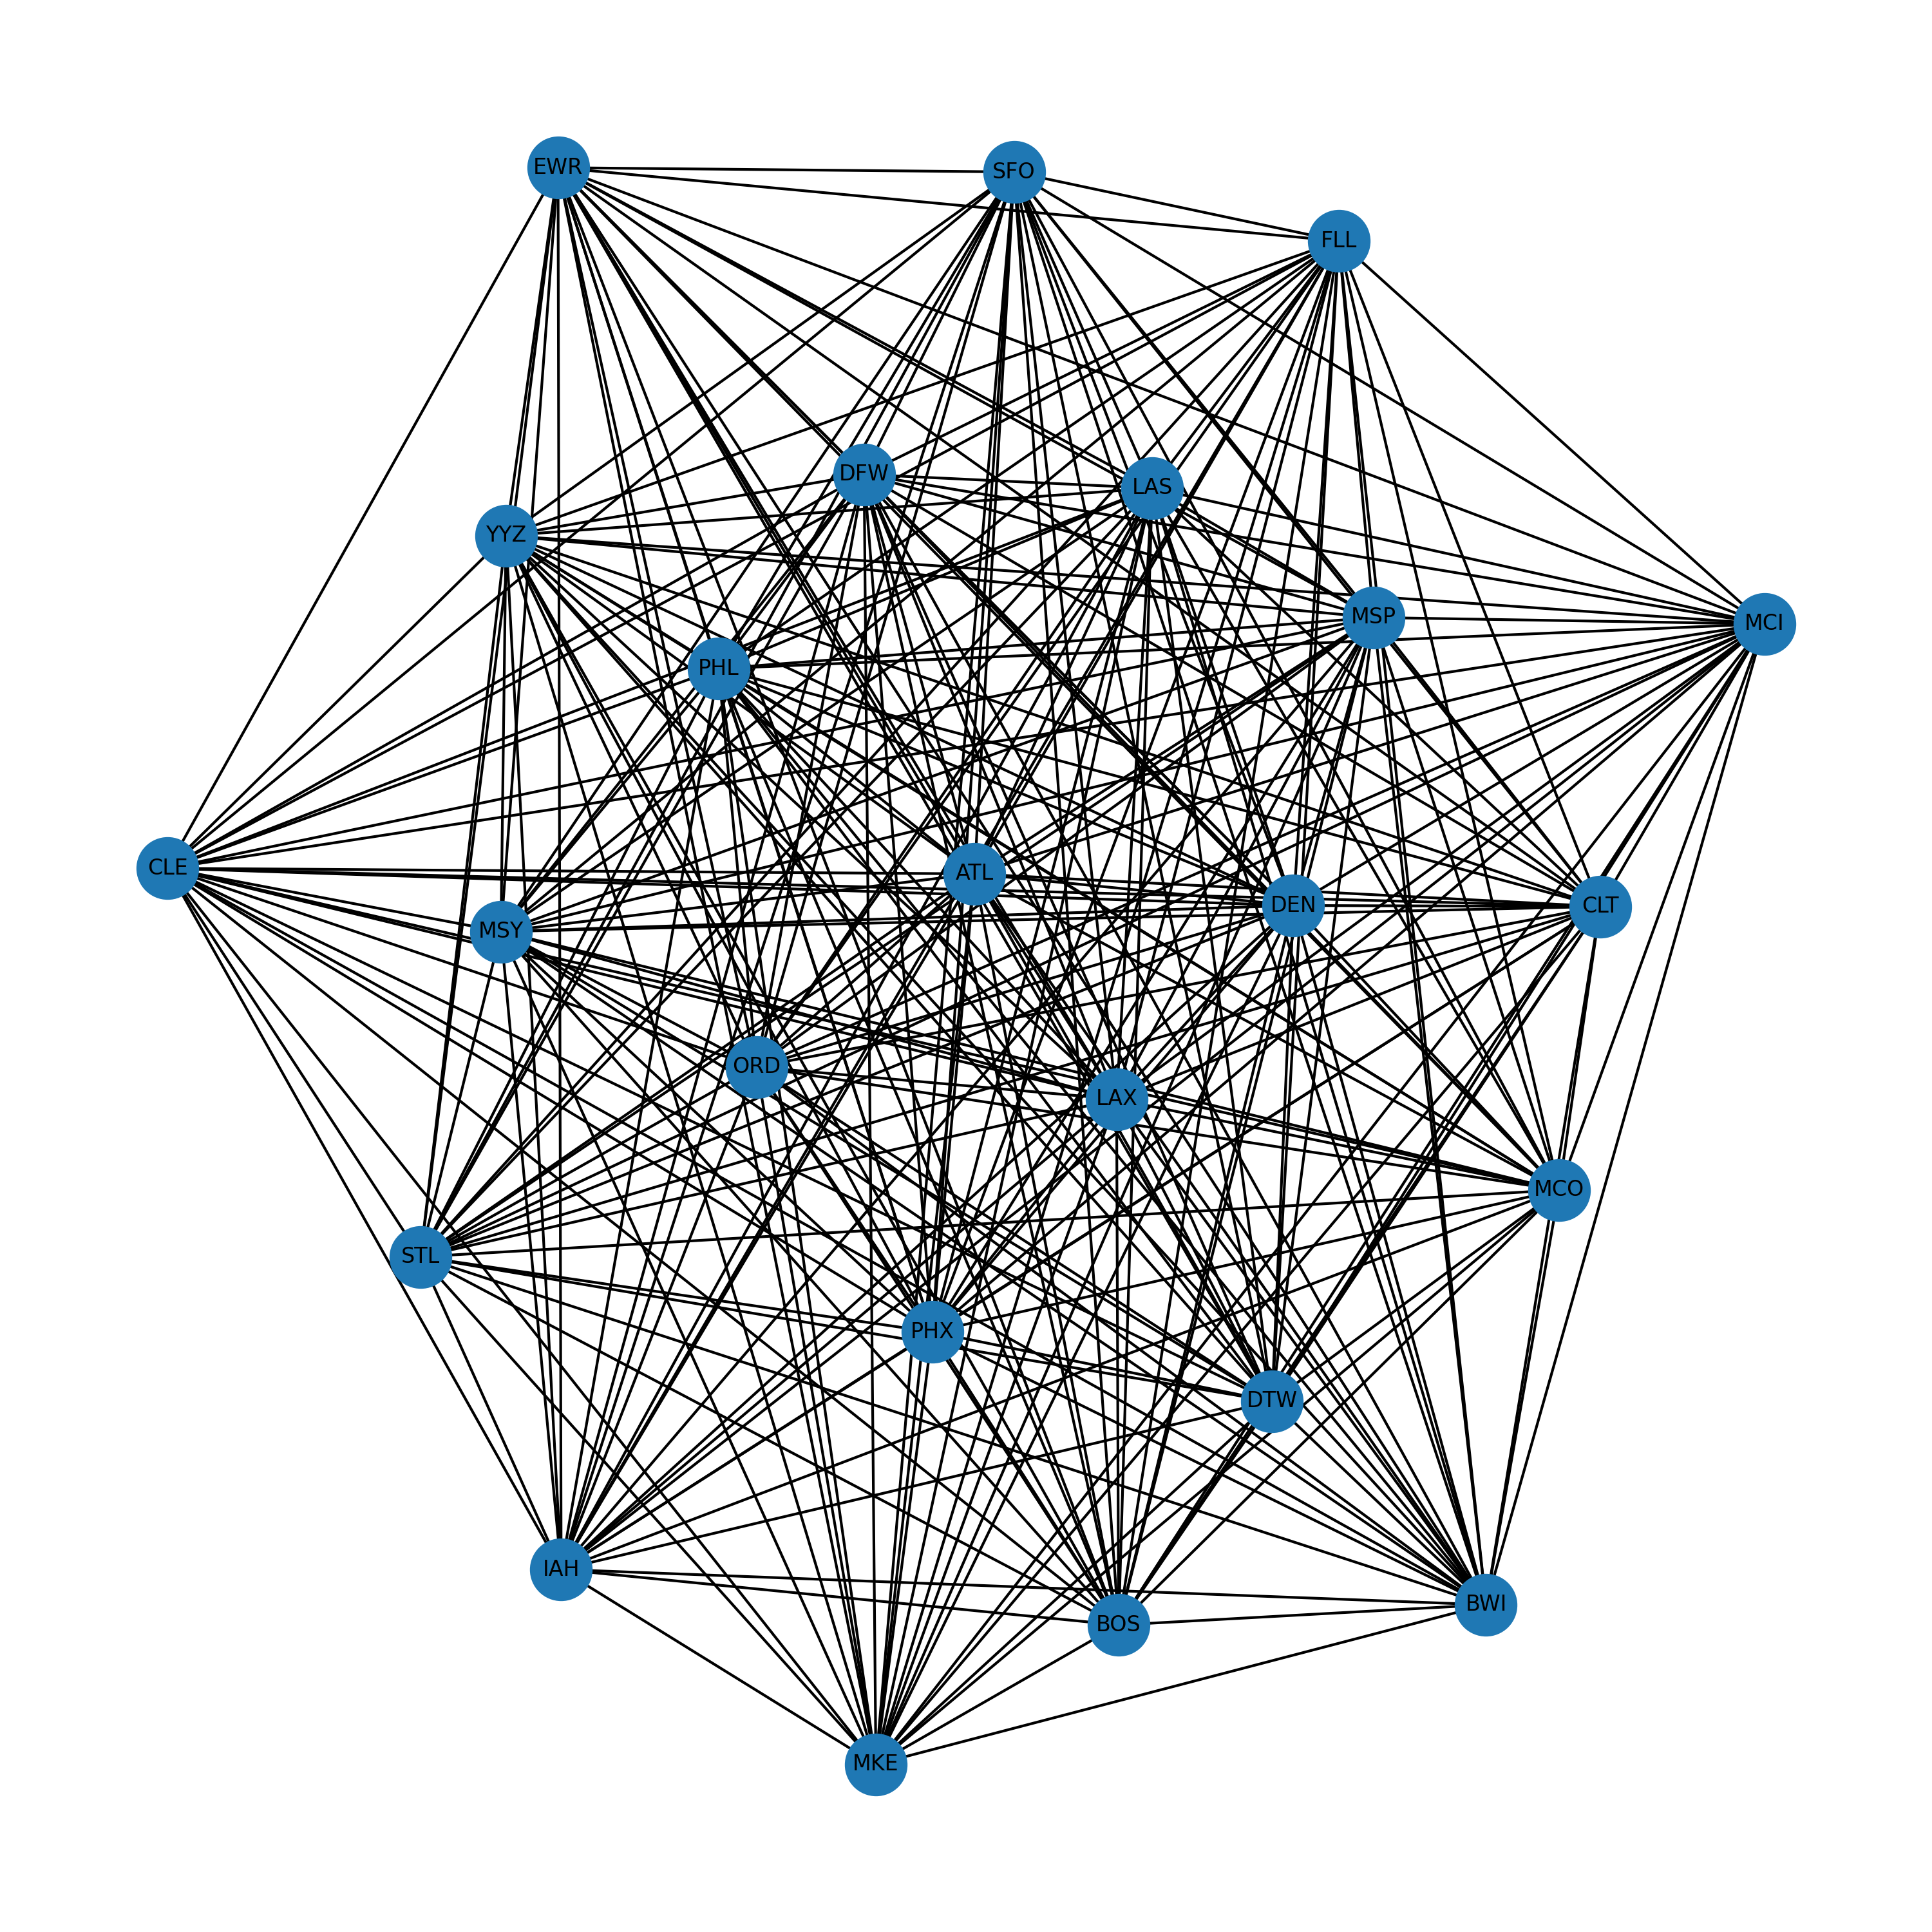
\includegraphics[width=0.9\textwidth]{chapter6/immagini/maximum_clique_graph.png}
\caption{Visualizzazione di una clique massima della rete.}
\label{fig:maximum_clique_graph}
\end{figure}

La Figura~\ref{fig:maximum_clique_graph} mostra una struttura estremamente densa e regolare, coerente con la definizione di clique. Anche dal punto di vista visivo, emerge chiaramente la forte coesione di questo sottografo, nel quale ogni aeroporto è direttamente collegato a tutti gli altri appartenenti alla stessa struttura.

\section{Sintesi dei principali risultati strutturali}

La Tabella~\ref{tab:structural_summary} riassume i principali risultati emersi dall’analisi delle strutture della rete.

\begin{table}[H]
\centering
\caption{Sintesi dei principali risultati dell’analisi strutturale della rete.}
\label{tab:structural_summary}
\begin{tabular}{lc}
\toprule
\textbf{Misura/struttura} & \textbf{Valore} \\
\midrule
Numero di community individuate & 19 \\
Dimensione community più grande & 659 \\
Massimo core number & 31 \\
Numero di nodi nel massimo k-core & 93 \\
Numero di archi nel massimo k-core & 2257 \\
Ego-network FRA: nodi & 245 \\
Ego-network FRA: archi & 4601 \\
Ego-network DXB: nodi & 189 \\
Ego-network DXB: archi & 2613 \\
Numero totale di clique massimali & 22763 \\
Dimensione massima di una clique & 24 \\
Numero di clique di dimensione massima & 2 \\
Clustering coefficient medio del grafo & 0.488336 \\
Clustering coefficient di FRA & 0.146968 \\
Clustering coefficient di DXB & 0.137957 \\
\bottomrule
\end{tabular}
\end{table}